\chapter{Thiết kế hệ thống}
\section{Kiến trúc tổng thể hệ thống}
\subsection{Kiến trúc N-tier}
\textbf{N-tier Architecture} (Kiến trúc đa tầng) là mô hình thiết kế phần mềm trong đó hệ thống được chia thành các tầng (layers) riêng biệt về mặt logic và vật lý.
\begin{itemize}
    \item \textbf{Nguyên tắc cốt lõi:} "Separation of Concerns" (Phân tách mối quan tâm). Mỗi tầng đảm nhiệm một chức năng cụ thể và chỉ giao tiếp với các tầng liền kề (thường là tầng ngay bên dưới nó).
    \item \textbf{Mục tiêu:} Giúp hệ thống dễ quản lý, dễ bảo trì, tăng tính bảo mật và khả năng mở rộng linh hoạt.
\end{itemize}
\subsection{Kết cấu chi tiết 5 Tầng (Structure)}
\subsubsection{Tầng 1: Presentation Layer (Client Layer)}
Đây là tầng giao diện người dùng, nơi tương tác trực tiếp với người dùng cuối (End-user).
\begin{itemize}
    \item \textbf{Chức năng:} Hiển thị thông tin và thu thập hành động của người dùng (click, nhập liệu). Nó không chứa logic nghiệp vụ phức tạp mà chỉ chịu trách nhiệm về UX/UI.
    \item \textbf{Thành phần:} Mobile App (iOS, Android, Flutter), Web App (React, Vue, Angular), hoặc Desktop App.
    \item \textbf{Giao tiếp:} Gửi yêu cầu (Request) xuống Tầng 2 và nhận phản hồi (Response) để hiển thị.
\end{itemize}
\subsubsection{Tầng 2: Connection \& API Layer (Gateway)}
Đây là "người gác cổng" (Gatekeeper) của hệ thống phía sau. Mọi yêu cầu từ Client phải đi qua đây trước khi vào hệ thống nội bộ.
\begin{itemize}
    \item \textbf{Chức năng:} \textbf{API Gateway:} Định tuyến (Routing) yêu cầu đến đúng service xử lý. \textbf{Security:} Xác thực (Authentication), Phân quyền (Authorization), chặn DDoS, Rate Limiting (giới hạn số lượt truy cập). \textbf{Load Balancing:} Cân bằng tải để phân phối request đều đặn.
    \item \textbf{Công nghệ:} NGINX, Kong, AWS API Gateway, Spring Cloud Gateway.
\end{itemize}
\subsubsection{Tầng 3: Business Logic Layer (Server Layer - Microservices)}
Đây là "bộ não" của hệ thống, nơi xử lý các quy trình nghiệp vụ chính. Trong kiến trúc hiện đại, tầng này thường được chia nhỏ thành các \textbf{Microservices}.
\begin{itemize}
    \item \textbf{Chức năng:} Xử lý tính toán, logic nghiệp vụ (ví dụ: tính toán giỏ hàng, kiểm tra tồn kho, xử lý workflow).
    \item \textbf{Đặc điểm:} Mỗi Microservice chạy độc lập, có thể viết bằng các ngôn ngữ khác nhau (Java, Go, Python, Node.js) và giao tiếp với nhau qua HTTP/REST hoặc gRPC.
    \item \textbf{Giao tiếp:} Nhận lệnh từ Tầng 2, gọi xuống Tầng 4 để lấy dữ liệu, hoặc gọi sang Tầng 5 để dùng dịch vụ bên ngoài.
\end{itemize}
\subsubsection{Tầng 4: Data Access Layer (Data \& Infrastructure Layer)}
Tầng này chịu trách nhiệm quản lý và lưu trữ dữ liệu bền vững. Tầng Business không bao giờ truy cập trực tiếp vào file database vật lý mà phải thông qua các cơ chế của tầng này.
\begin{itemize}
    \item \textbf{Chức năng:}
        \begin{itemize}
            \item Thực hiện các thao tác CRUD (Create, Read, Update, Delete).
            \item Trừu tượng hóa việc truy cập dữ liệu (giúp Tầng 3 không cần biết chi tiết kỹ thuật của Database).
            \item Quản lý kết nối đến Database.
           
        \end{itemize}
   \item \textbf{Thành phần:} ORM (Entity Framework, Hibernate), SQL Database (PostgreSQL, MySQL), NoSQL (MongoDB), Caching (Redis).
    
\end{itemize}
\subsubsection{Tầng 5: Integration Layer (Third-Party Integrations)}
Đây là tầng kết nối với thế giới bên ngoài, giúp hệ thống mở rộng chức năng mà không cần tự xây dựng lại từ đầu.
\begin{itemize}
    \item \textbf{Chức năng:}
    \begin{itemize}
        \item Đóng vai trò là "Adapter" để kết nối hệ thống nội bộ với các dịch vụ thuê ngoài.
        \item Xử lý việc chuyển đổi định dạng dữ liệu để phù hợp với API của đối tác.
    \end{itemize}
    \item \textbf{Thành phần:}  Payment Gateway (Stripe, Momo), SMS/Email Services (Twilio, SendGrid), Maps API, AI Services.
\end{itemize}

\subsection{Ưu điểm và Nhược điểm}
\begin{table}[htbp]
    \centering
    \caption{Ưu điểm và Nhược điểm của Kiến trúc Layer (N-tier)}
    \label{tab:ntier-comparison}
    \renewcommand{\arraystretch}{1.5} % Tăng khoảng cách giữa các dòng cho dễ đọc
    
    % Tạo bảng với 2 cột có độ rộng bằng nhau (X)
    \begin{tabularx}{\textwidth}{ | >{\raggedright\arraybackslash}X | >{\raggedright\arraybackslash}X | }
        \hline
        \textbf{Ưu điểm (Advantages)} & \textbf{Nhược điểm (Disadvantages)} \\  
        \hline
        
        \textbf{1. Khả năng mở rộng (Scalability):} \newline 
        Có thể mở rộng (scale-out) từng tầng riêng biệt. Ví dụ: Nếu Business Layer quá tải, chỉ cần thêm server cho tầng này mà không cần can thiệp vào Database hay Client. 
        & 
        \textbf{1. Độ trễ (Latency):} \newline 
        Hiệu năng có thể bị ảnh hưởng do dữ liệu phải di chuyển qua nhiều tầng (network hops) và các lớp bảo mật trước khi đến đích, chậm hơn so với kiến trúc nguyên khối. \\  
        \hline
        
        \textbf{2. Dễ bảo trì (Maintainability):} \newline 
        Nhờ nguyên tắc "Separation of Concerns", việc sửa lỗi hoặc nâng cấp công nghệ ở một tầng ít gây ảnh hưởng đến các tầng khác (Loose Coupling). 
        & 
        \textbf{2. Phức tạp trong vận hành:} \newline 
        Việc triển khai (deployment), giám sát (monitoring) và gỡ lỗi (debugging) trở nên khó khăn hơn vì hệ thống bị phân tán thành nhiều phần. \\  
        \hline
        
        \textbf{3. Bảo mật cao (Security):} \newline 
        Tầng dữ liệu (Data Layer) và Business Layer được che giấu sau Gateway. Kẻ tấn công khó tiếp cận trực tiếp vào cơ sở dữ liệu. 
        & 
        \textbf{3. Chi phí hạ tầng cao:} \newline 
        Yêu cầu nhiều tài nguyên server, chi phí quản lý mạng và license phần mềm để duy trì nhiều tầng riêng biệt. \\  
        \hline
        
        \textbf{4. Linh hoạt công nghệ:} \newline 
        Tầng Presentation có thể dùng Flutter/React, trong khi Business Layer có thể dùng song song Java, Go hoặc Python. 
        & 
        \textbf{4. Tính nhất quán dữ liệu:} \newline 
        Trong mô hình Microservices, việc đảm bảo dữ liệu đồng bộ giữa các service (Data Consistency) phức tạp hơn, cần các pattern nâng cao như Saga. \\  
        \hline
        
    \end{tabularx}
\end{table}

\subsection{Các Kiến trúc Thay thế và So sánh}
\begin{table}[htbp]
    \centering
    \caption{So sánh Kiến trúc N-tier với các Kiến trúc khác}
    \vspace{0.3cm}
    \renewcommand{\arraystretch}{1.5} % Khoảng cách dòng
    
    % --- CHỈNH SỬA TỶ LỆ CỘT TẠI ĐÂY ---
    % Tổng các hệ số hsize phải bằng 4 (số lượng cột X)
    % Cột 1: 0.8 (Tăng lên để chứa chữ Microservices/Orchestration không bị ngắt)
    % Cột 2: 0.6 (Giữ nguyên)
    % Cột 3: 1.3 (Giảm nhẹ để bù cho cột 1)
    % Cột 4: 1.3 (Giảm nhẹ để bù cho cột 1)
    \begin{tabularx}{\textwidth}{ 
        | >{\hsize=0.8\hsize\RaggedRight\arraybackslash}X 
        | >{\hsize=0.6\hsize\RaggedRight\arraybackslash}X 
        | >{\hsize=1.3\hsize\RaggedRight\arraybackslash}X 
        | >{\hsize=1.3\hsize\RaggedRight\arraybackslash}X | }
        
        \hline
        \textbf{So với} & \textbf{Tiêu chí} & \textbf{Ưu điểm N-tier} & \textbf{Nhược điểm N-tier} \\  
        \hline

        % --- CQRS ---
        \textbf{CQRS} & 
        Tách biệt Đọc/Ghi & 
        \textbf{Đơn giản:} Dùng chung model cho đọc/ghi giúp triển khai nhanh, code dễ hiểu, phù hợp đa số ứng dụng. & 
        \textbf{Hiệu năng truy vấn:} Khó tối ưu các báo cáo phức tạp so với database chuyên dụng cho việc đọc của CQRS. \\  
        \hline

        % --- Microservices ---
        \textbf{Microservices} & 
        Phạm vi triển khai & 
        \textbf{Dễ quản lý hạ tầng:} Ít phức tạp về mạng lưới. Test tích hợp (End-to-End) dễ hơn do luồng đi thẳng. & 
        \textbf{Khó scale cục bộ:} Phải scale cả tầng lớn thay vì từng service nhỏ. Khả năng cô lập lỗi kém hơn. \\  
        \hline

        % --- Orchestration ---
        \textbf{Orchestration} & 
        Quản lý quy trình & 
        \textbf{Luồng rõ ràng:} Dễ theo dõi (trace) luồng đi từ Client xuống DB. Tốt cho tác vụ đồng bộ. & 
        \textbf{Phình to Logic:} Dễ dẫn đến "Business Layer" quá tải khi quy trình nghiệp vụ trở nên chằng chịt. \\  
        \hline

        % --- MVP ---
        \textbf{MVP} & 
        Phạm vi kiến trúc & 
        \textbf{Vĩ mô:} N-tier giải quyết cấu trúc toàn hệ thống (Server/DB), trong khi MVP chỉ lo phần giao diện (UI). & 
        \textbf{Coupling:} Nếu không khéo, logic nghiệp vụ dễ bị dính chặt vào code giao diện hơn so với MVP thuần. \\  
        \hline

        % --- Event-Driven ---
        \textbf{Event-Driven} & 
        Giao tiếp & 
        \textbf{Nhất quán tức thì:} Xử lý đồng bộ giúp User biết ngay kết quả (thành công/thất bại). Dễ debug. & 
        \textbf{Chặn (Blocking):} Request phải chờ xử lý xong, dễ gây nghẽn cổ chai nếu tải cao so với xử lý ngầm. \\  
        \hline

    \end{tabularx}
\end{table}

\subsection{Diagram và Kết luận}
\begin{figure}[H]
    % Căn giữa hình ảnh
    \centering
    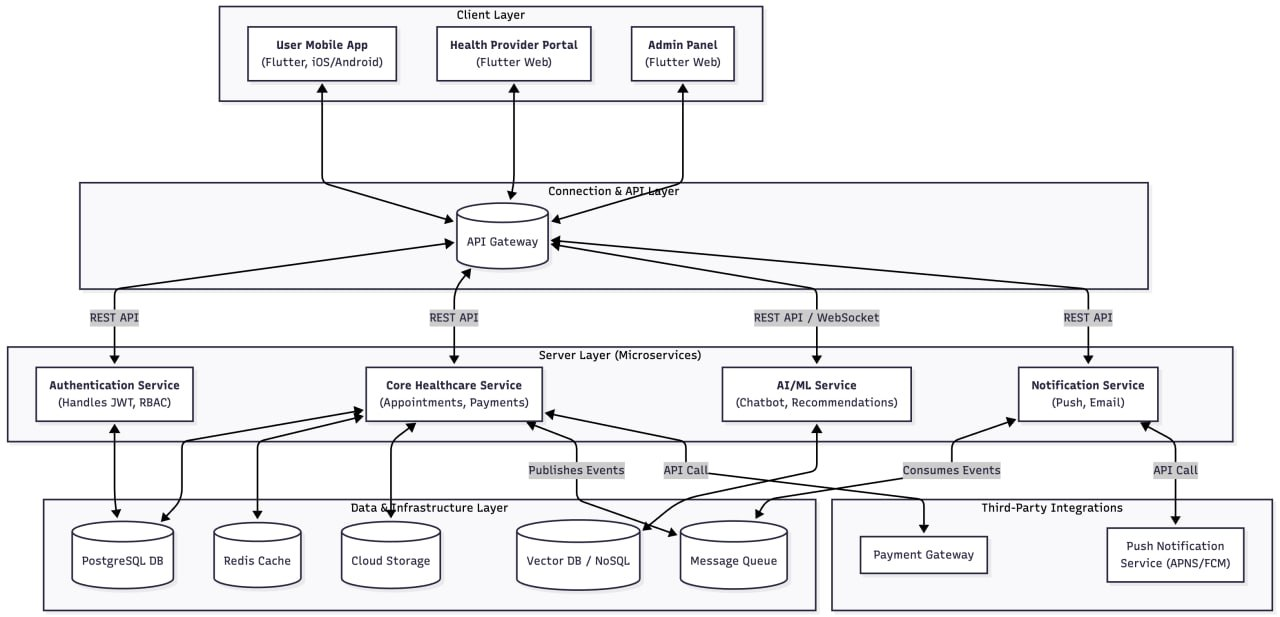
\includegraphics[width=1\textwidth]{Images/ArchSys.png}
    \vspace{10pt}
    
    % Thêm chú thích cho hình ảnh
    \caption{Kiến trúc hệ thống}
    
    % Đặt nhãn để tham chiếu chéo (cross-reference)
    \label{fig:sys_arch}
\end{figure}
Dựa trên hình ảnh \ref{fig:sys_arch}, kiến trúc tổng thể của hệ thống được thiết kế theo mô hình Microservices, chia thành 5 tầng chính (layer) với chức năng cụ thể như sau:
\begin{enumerate}
    \item \textbf{Client Layer (Tầng người dùng):}
    Đây là điểm tương tác trực tiếp với người dùng cuối và quản trị viên. Tầng này bao gồm ba ứng dụng chính được phát triển trên nền tảng Flutter:
    \begin{itemize}
        \item \textit{User Mobile App:} Ứng dụng di động (iOS/Android) dành cho khách hàng/bệnh nhân.
        \item \textit{Health Provider Portal:} Cổng thông tin dạng Web dành cho các nhà cung cấp dịch vụ y tế.
        \item \textit{Admin Panel:} Trang quản trị dạng Web để vận hành hệ thống.
    \end{itemize}

    \item \textbf{Connection \& API Layer (Tầng kết nối):}
    Đóng vai trò là cổng trung gian (Middleware) duy nhất giao tiếp giữa Client và Server.
    \begin{itemize}
        \item \textit{API Gateway:} Tiếp nhận toàn bộ yêu cầu (request) từ phía Client, thực hiện định tuyến (routing) đến các dịch vụ (services) phù hợp bên dưới.
    \end{itemize}

    \item \textbf{Server Layer (Tầng dịch vụ - Microservices):}
    Trung tâm xử lý logic nghiệp vụ, được chia nhỏ thành các dịch vụ độc lập giao tiếp qua REST API hoặc WebSocket:
    \begin{itemize}
        \item \textit{Authentication Service:} Quản lý xác thực và phân quyền (xử lý JWT, RBAC).
        \item \textit{Core Healthcare Service:} Xử lý các nghiệp vụ cốt lõi như đặt lịch khám, thanh toán. Dịch vụ này có khả năng công bố (publish) sự kiện.
        \item \textit{AI/ML Service:} Cung cấp các tính năng thông minh như Chatbot và gợi ý (Recommendations), hỗ trợ giao tiếp thời gian thực qua WebSocket.
        \item \textit{Notification Service:} Quản lý việc gửi thông báo (Push notification, Email) tới người dùng.
    \end{itemize}

    \item \textbf{Data \& Infrastructure Layer (Tầng dữ liệu và hạ tầng):}
    Nơi lưu trữ và quản lý dữ liệu bền vững, bao gồm:
    \begin{itemize}
        \item \textit{PostgreSQL DB:} Cơ sở dữ liệu quan hệ cho dữ liệu nghiệp vụ chính.
        \item \textit{Redis Cache:} Bộ nhớ đệm giúp tăng tốc độ truy xuất dữ liệu.
        \item \textit{Cloud Storage:} Lưu trữ tài liệu, hình ảnh.
        \item \textit{Vector DB / NoSQL:} Hỗ trợ lưu trữ dữ liệu phi cấu trúc phục vụ cho AI/ML.
        \item \textit{Message Queue:} Hàng đợi thông điệp giúp xử lý bất đồng bộ và giao tiếp giữa các services (Event-driven).
    \end{itemize}

    \item \textbf{Third-Party Integrations (Tầng tích hợp bên thứ ba):}
    Các dịch vụ bên ngoài được hệ thống kết nối để mở rộng tính năng:
    \begin{itemize}
        \item \textit{Payment Gateway:} Cổng thanh toán trực tuyến.
        \item \textit{Push Notification Service (APNS/FCM):} Dịch vụ đẩy thông báo của Apple và Google.
    \end{itemize}
\end{enumerate}
\section{Thiết kế cơ sở dữ liệu}
\subsection{Mô tả}
Thực thể (ERD) được cung cấp, nhằm mục đích làm rõ cấu trúc dữ liệu và các phân hệ chức năng chính của hệ thống. Mô hình dữ liệu cho thấy đây là một nền tảng công nghệ được thiết kế để kết nối ba nhóm đối tượng chính: Người dùng cuối (Khách hàng), Đối tác cung cấp dịch vụ (Partner), và Nhân viên quản trị (Employee).
\subsection{Các khối chức năng chính}
 Dựa trên các thực thể và mối quan hệ trong sơ đồ, hệ thống được cấu thành từ các khối chức năng (module) chính sau:
 \begin{itemize}
            \item Module Quản lý Tài khoản và Phân quyền (Account Management)
            Đây là module lõi, quản lý định danh và quyền truy cập của toàn bộ người dùng trên hệ thống.
            \begin{itemize}
                \item Thực thể trung tâm: \textbf{Account} lưu trữ thông tin xác thực chung
                \item Cơ chế phân quyền: Hệ thống định nghĩa ba vai trò người dùng riêng biệt với các quyền hạn khác nhau:
                \begin{itemize}
                    \item User: Đối tượng sử dụng dịch vụ.
                    \item Partner: Đối tượng cung cấp dịch vụ/sản phẩm.
                    \item Employee: Đối tượng quản trị và vận hành nền tảng.
                \end{itemize}
                \item Chức năng: Cung cấp cơ chế đăng ký, đăng nhập, xác thực và phân quyền truy cập chức năng tương ứng với từng vai trò.
            \end{itemize}
            \item \textbf{Phân hệ Vận hành dành cho Đối tác (Partner Portal)}: 
            Phân hệ này cung cấp một cổng quản trị toàn diện, cho phép các đối tác số hóa và quản lý hoạt động kinh doanh của mình.
            \begin{itemize}
                \item Quản lý Dịch vụ \& Sản phẩm (Service, Product): Cho phép đối tác khởi tạo, cấu hình giá, mô tả và phân loại các dịch vụ/sản phẩm cung cấp. Thực thể Category giúp hệ thống hóa và hỗ trợ tìm kiếm hiệu quả.
                \item Quản lý Nhân sự (Employee của Partner): Hỗ trợ đối tác quản lý thông tin nhân viên thực hiện dịch vụ.
                \item Quản lý Lịch trình (Schedule): Cung cấp công cụ thiết lập lịch làm việc cho cơ sở và từng nhân viên, làm cơ sở cho tính năng đặt lịch.
            \end{itemize}
        \item \textbf{Phân hệ Trải nghiệm Người dùng (User Experience)} Phân hệ này xây dựng luồng tương tác hoàn chỉnh cho khách hàng cuối.
            \begin{itemize}
                \item Đặt lịch (Booking): Là nghiệp vụ cốt lõi, liên kết các thực thể chính: User, Partner, Service, và Employee (của Partner) tại một thời điểm cụ thể. Trạng thái của lịch hẹn (ví dụ: chờ xác nhận, đã hoàn thành, đã hủy) cũng được quản lý tại đây.
            \item Tìm kiếm và Khám phá: Cấu trúc dữ liệu cho phép người dùng truy vấn, lọc và tìm kiếm dịch vụ/đối tác dựa trên nhiều tiêu chí.
            \item Phản hồi và Đánh giá (Feedback/Review): Sau khi sử dụng dịch vụ, người dùng có thể cung cấp phản hồi, giúp xây dựng độ tin cậy và là cơ sở để đánh giá chất lượng đối tác. 
            \end{itemize}
        \item \textbf{Module Tài chính và Marketing}
        Module này tích hợp các nghiệp vụ liên quan đến giao dịch và các hoạt động thu hút người dùng.
            \begin{itemize}
                \item Xử lý Thanh toán (Payment): Mỗi thực thể Booking được liên kết với một giao dịch Payment, ghi nhận các thông tin về số tiền, phương thức và trạng thái thanh toán.
                \item Quản lý Khuyến mãi (Promotion\(\)Voucher): Cung cấp chức năng tạo và quản lý các chương trình khuyến mãi. Các chương trình này có thể được áp dụng vào giao dịch Booking để điều chỉnh giá trị thanh toán cuối cùng.
            \end{itemize}
        \end{itemize}
\subsection{Kết luận}
Sơ đồ ERD mô tả một cấu trúc dữ liệu chặt chẽ và toàn diện cho một nền tảng dịch vụ đa năng. Từ phân tích trên, có thể xác định các năng lực chính của hệ thống bao gồm:
    \begin{itemize}
        \item Hệ thống quản lý người dùng đa vai trò với cơ chế phân quyền rõ ràng.
        \item Nền tảng đặt lịch (booking platform) thông minh, kết nối nhu cầu của người dùng với khả năng cung ứng của đối tác.
        \item Cổng quản trị dành cho đối tác (partner portal) để tự quản lý vận hành kinh doanh.
        \item Cơ chế thanh toán và khuyến mãi tích hợp, hỗ trợ hoàn chỉnh vòng đời giao dịch và các hoạt động marketing.
        \item Hệ thống thu thập phản hồi và đánh giá, đảm bảo chất lượng và tính minh bạch của nền tảng.
    \end{itemize}
\subsection{Lược đồ}
\begin{figure}[H]
    % Căn giữa hình ảnh
    \centering
    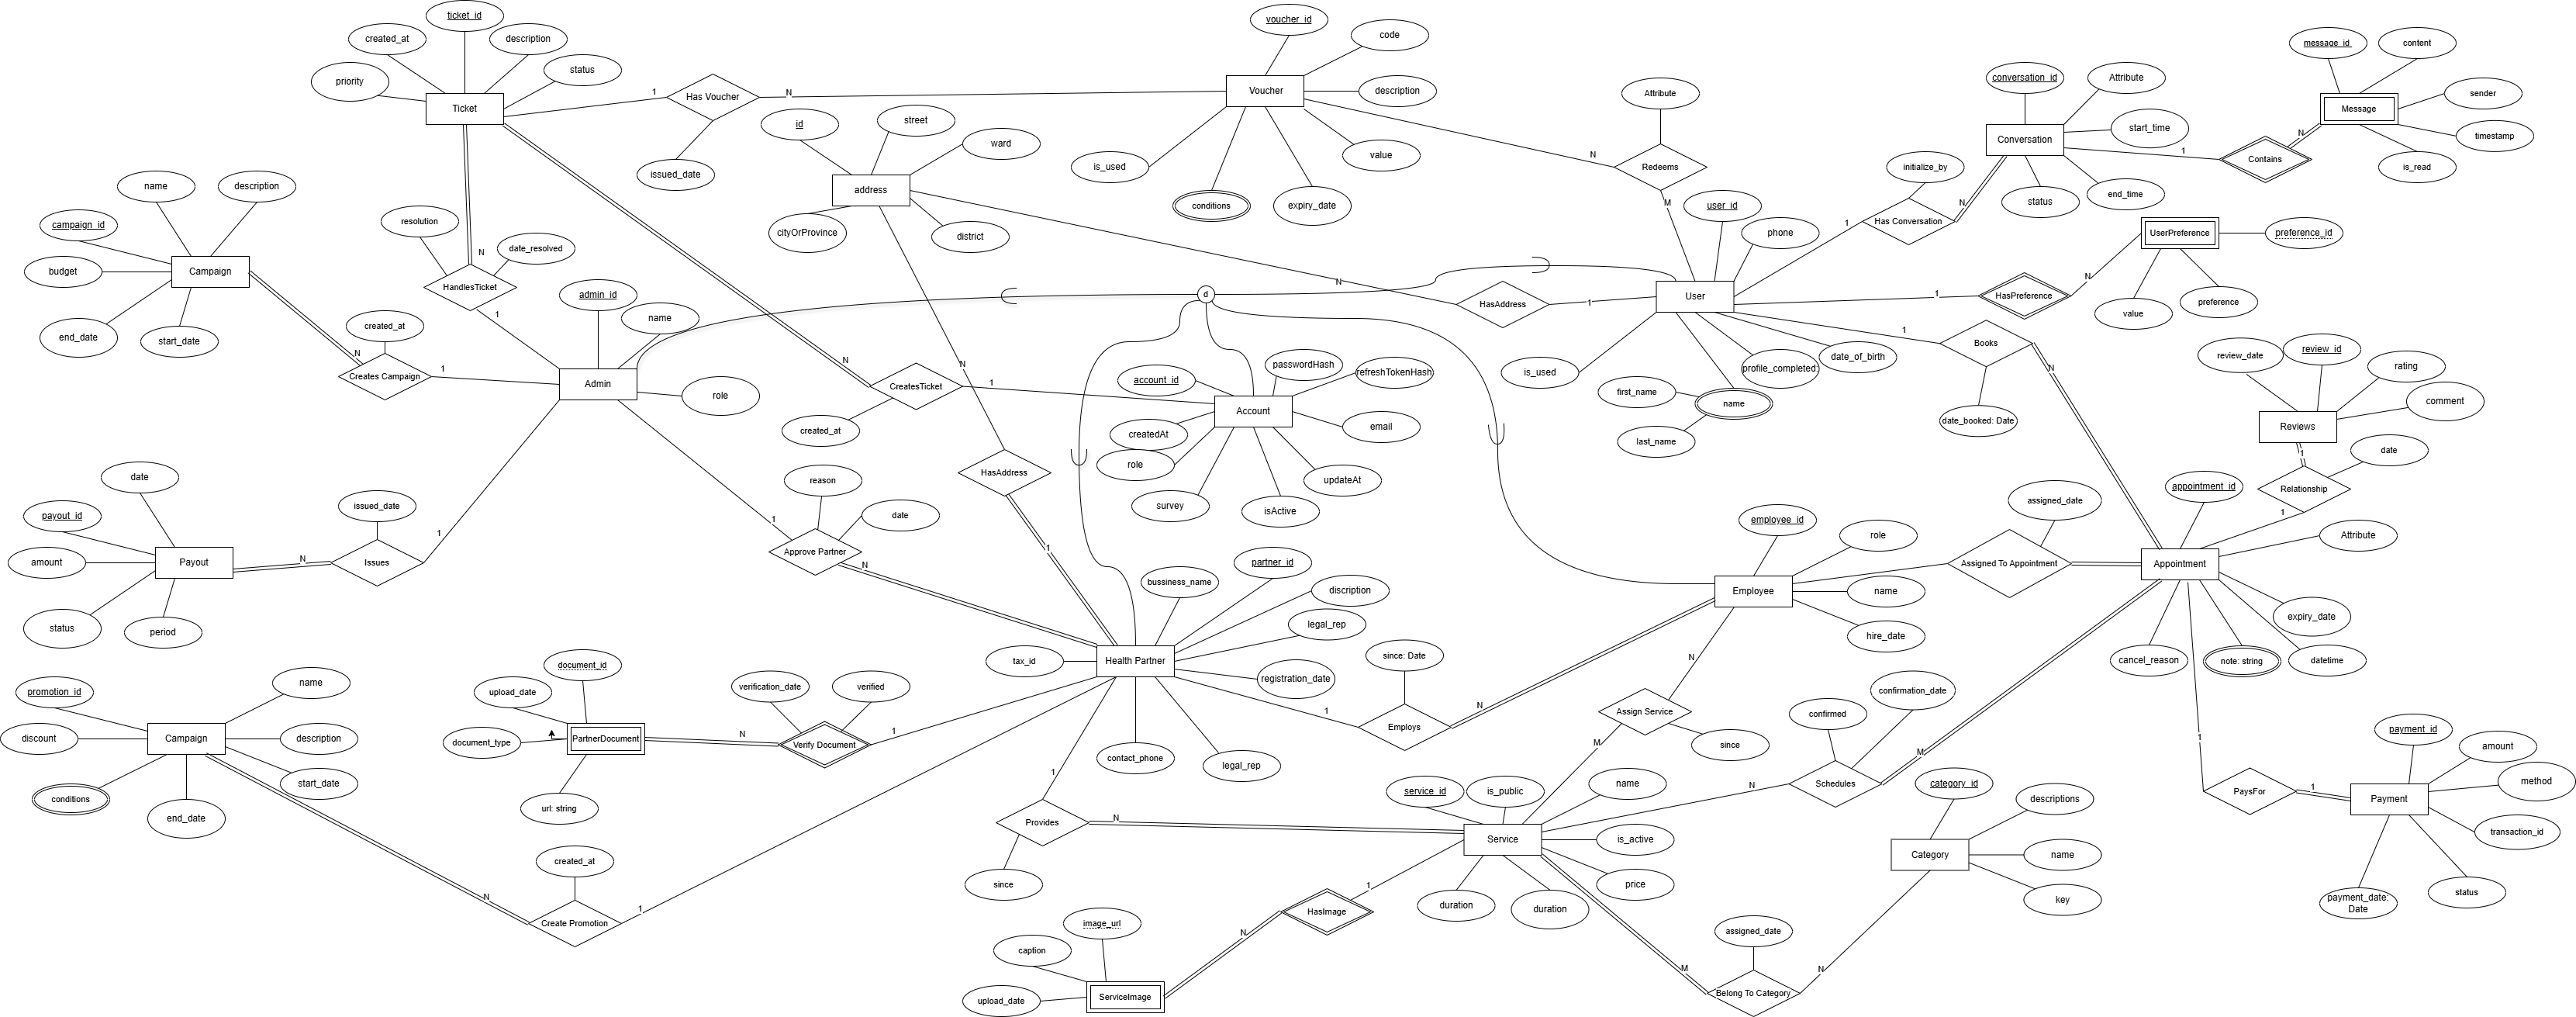
\includegraphics[angle=-90, width=0.6\textwidth]{Images/ERD.png}
    \vspace{10pt}
    
    % Thêm chú thích cho hình ảnh
    \caption{ER Diagram của hệ thống}
    
    % Đặt nhãn để tham chiếu chéo (cross-reference)
    \label{fig:erd}
\end{figure}


\section{Thiết kế UI/UX cơ bản}

\subsection{Mockup UI - Tổng quan giao diện}
Sơ đồ mockup UI dưới đây thể hiện tổng quan luồng điều hướng và các màn hình chính của ứng dụng di động Healytics. Wireframe này được thiết kế để minh họa trải nghiệm người dùng từ khi đăng nhập cho đến khi sử dụng các tính năng cốt lõi của hệ thống.

\begin{figure}[H]
    \centering
    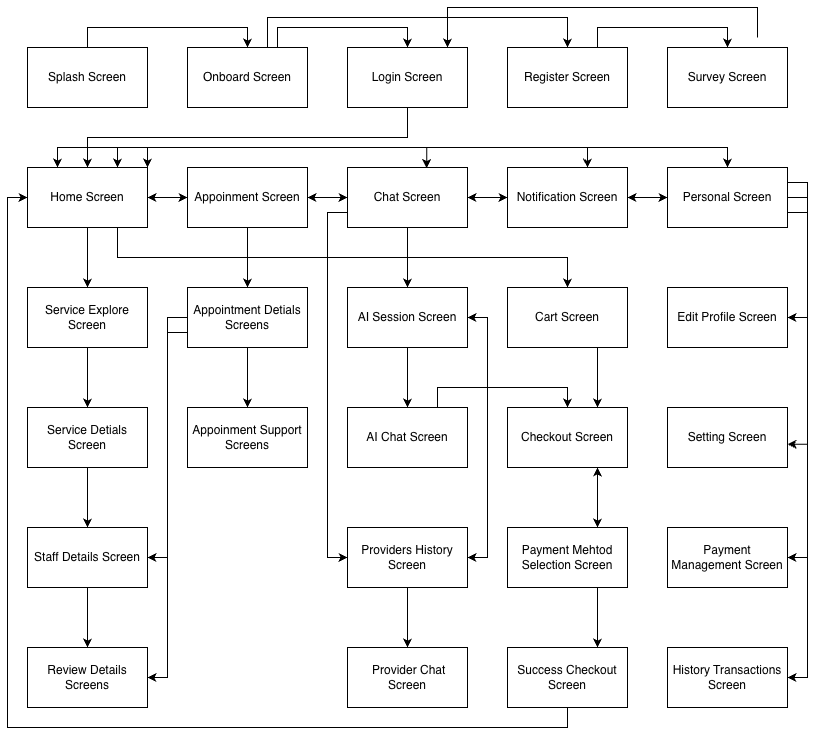
\includegraphics[width=1\textwidth]{Images/uiux/mock_ui.drawio.png}
    \vspace{10pt}
    \caption{Sơ đồ Mockup UI tổng quan của ứng dụng}
    \label{fig:mockup_ui_overview}
\end{figure}

Mockup bao gồm các nhóm màn hình chính:
\begin{itemize}
    \item \textbf{Authentication Flow:} Luồng xác thực bao gồm các màn hình đăng nhập, đăng ký qua email, xác thực OTP và các bước điền thông tin cá nhân.
    \item \textbf{Survey Flow:} Chuỗi các bước khảo sát thu thập thông tin sức khỏe và sở thích của người dùng để cá nhân hóa trải nghiệm.
    \item \textbf{Main Navigation:} Các màn hình điều hướng chính bao gồm Trang chủ (Home), Khám phá dịch vụ (Explore), Thông báo (Notification), và Trang cá nhân (Profile).
    \item \textbf{Appointment Booking:} Luồng đặt lịch hẹn khám bệnh với các bước chọn dịch vụ, thời gian, và xác nhận thông tin.
    \item \textbf{Provider \& Service Details:} Các màn hình hiển thị thông tin chi tiết về nhà cung cấp dịch vụ y tế và các dịch vụ cụ thể.
    \item \textbf{AI Chat Assistant:} Giao diện trợ lý AI hỗ trợ người dùng tư vấn sức khỏe thông qua hội thoại tự nhiên.
\end{itemize}

Các phần tiếp theo trình bày chi tiết thiết kế giao diện cho các nhóm chức năng cốt lõi. Các nhóm chức năng bổ sung (Survey, Provider Service, Checkout) được trình bày đầy đủ tại \textbf{Phụ lục A}.

\subsection{Authentication - Đăng nhập \& Đăng ký}
\begin{figure}[H]
    \centering
    
    % --- Hàng 1 ---
    \begin{subfigure}[b]{0.24\textwidth}
        \centering
        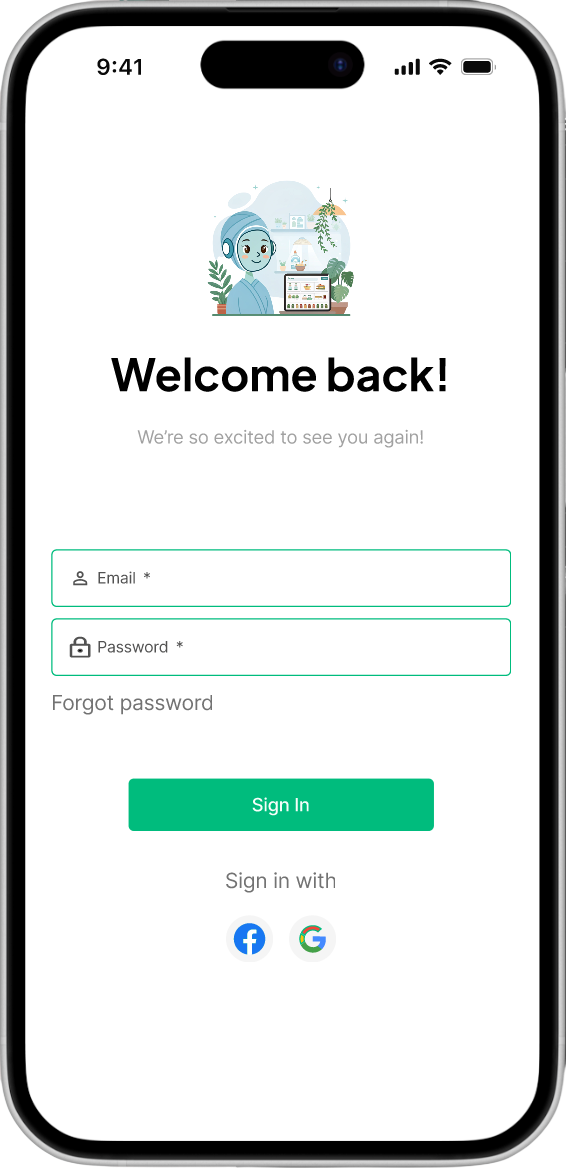
\includegraphics[width=\linewidth]{Images/uiux/authen/login.png}
        \caption{Login Page}
    \end{subfigure}
    \hfill
    \begin{subfigure}[b]{0.24\textwidth}
        \centering
        
\includegraphics[width=\linewidth]{Images/uiux/authen/signup_email.png}
        \caption{Sign Up Email}
    \end{subfigure}
    \hfill
    \begin{subfigure}[b]{0.24\textwidth}
        \centering
        
\includegraphics[width=\linewidth]{Images/uiux/authen/signup_otp.png}
        \caption{Sign Up OTP}
    \end{subfigure}
    \hfill
    \begin{subfigure}[b]{0.24\textwidth}
        \centering
        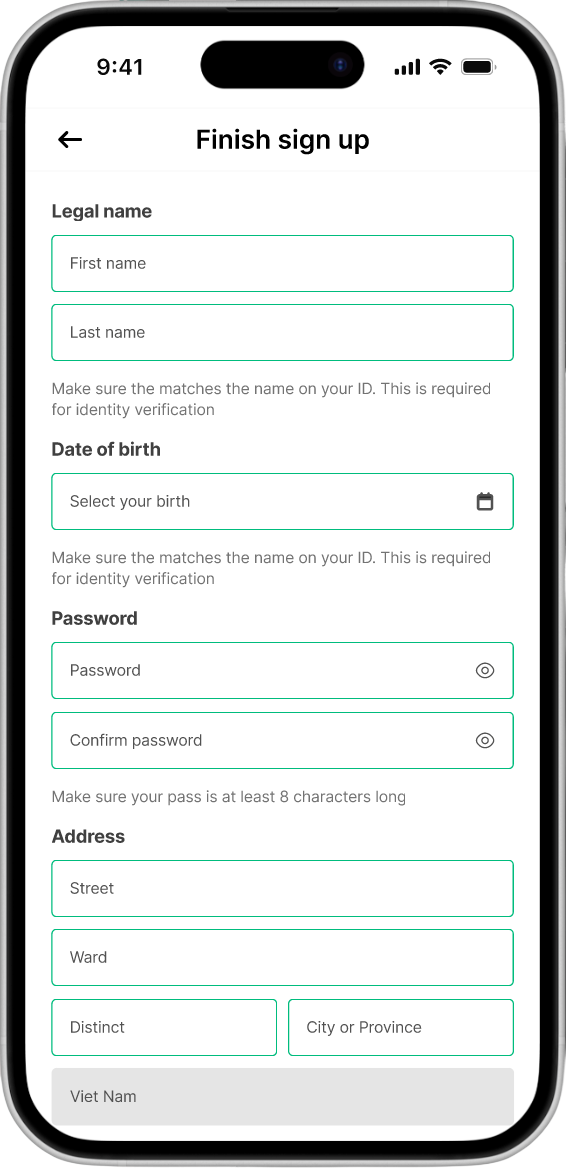
\includegraphics[width=\linewidth]{Images/uiux/authen/signup_form1.png}
        \caption{Sign Up Form 1}
    \end{subfigure}
    
    \vspace{1em}
    
    % --- Hàng 2 ---
    \begin{subfigure}[b]{0.24\textwidth}
        \centering
        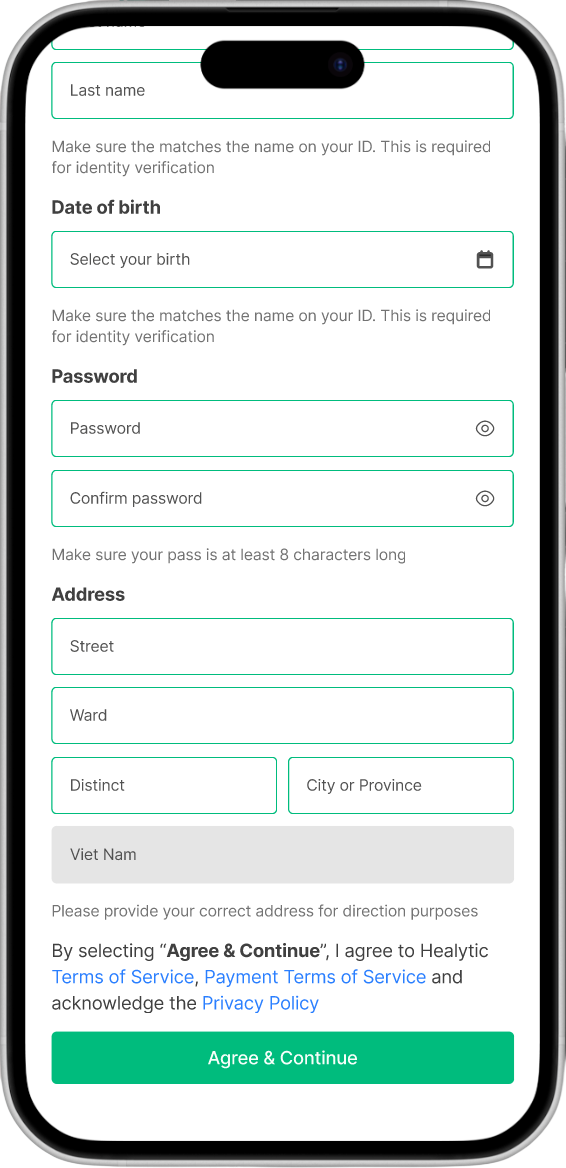
\includegraphics[width=\linewidth]{Images/uiux/authen/signup_form2.png}
        \caption{Sign Up Form 2}
    \end{subfigure}
    \hfill
    \begin{subfigure}[b]{0.24\textwidth}
        \centering
        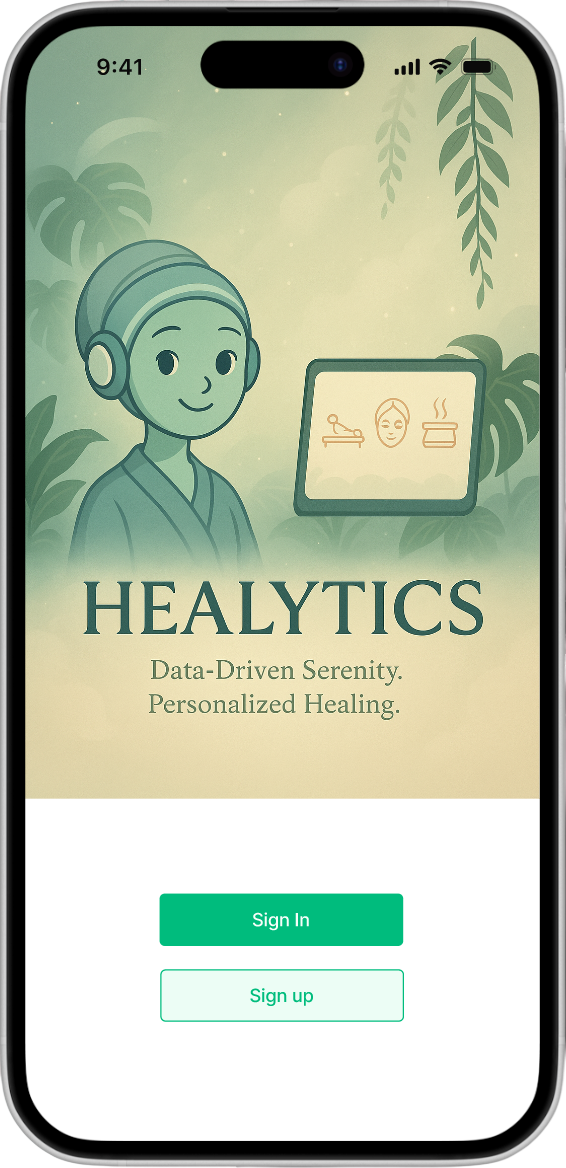
\includegraphics[width=\linewidth]{Images/uiux/authen/dashboard.png}
        \caption{Dashboard}
    \end{subfigure}
    \hfill
    \begin{subfigure}[b]{0.24\textwidth}
    \end{subfigure}
    \hfill
    \begin{subfigure}[b]{0.24\textwidth}
    \end{subfigure}
    
    \vspace{1em}
    \caption{Giao diện Authentication}
\end{figure}

\subsection{Navigation - Các trang điều hướng chính}
\begin{figure}[H]
    \centering
    
    % --- Hàng 1 ---
    \begin{subfigure}[b]{0.24\textwidth}
        \centering
        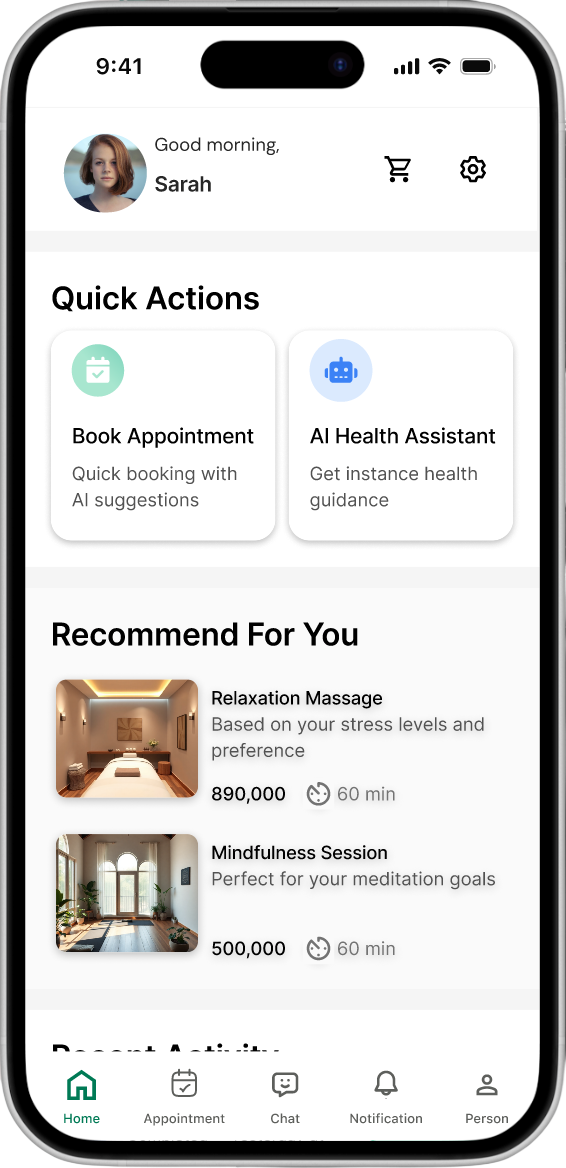
\includegraphics[width=\linewidth]{Images/uiux/navigation/home_1.png}
        \caption{Home Page 1}
    \end{subfigure}
    \hfill
    \begin{subfigure}[b]{0.24\textwidth}
        \centering
        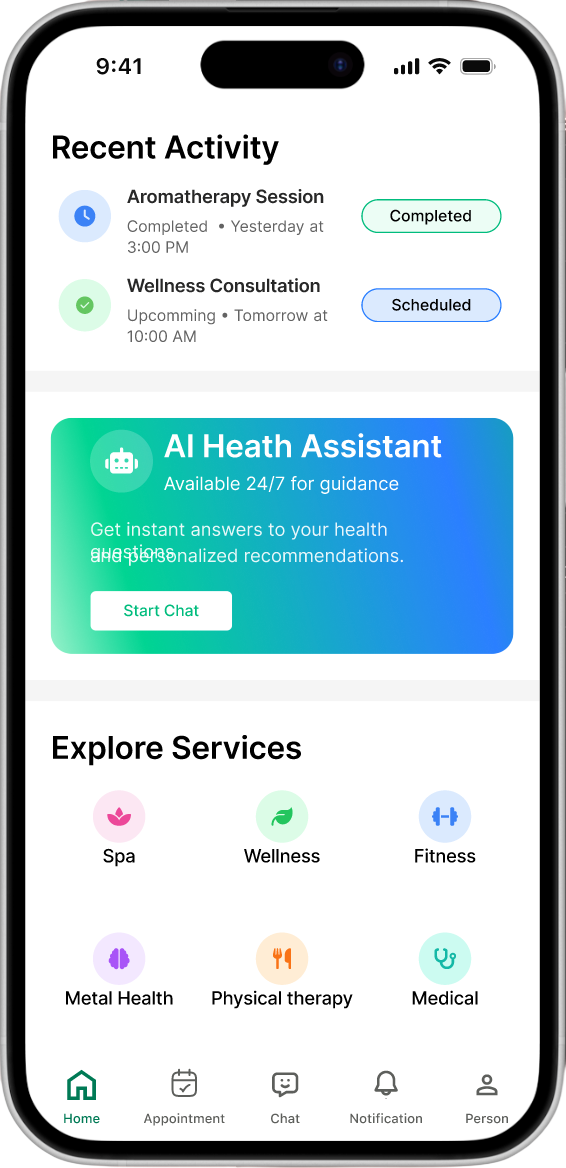
\includegraphics[width=\linewidth]{Images/uiux/navigation/home_2.png}
        \caption{Home Page 2}
    \end{subfigure}
    \hfill
    \begin{subfigure}[b]{0.24\textwidth}
        \centering
        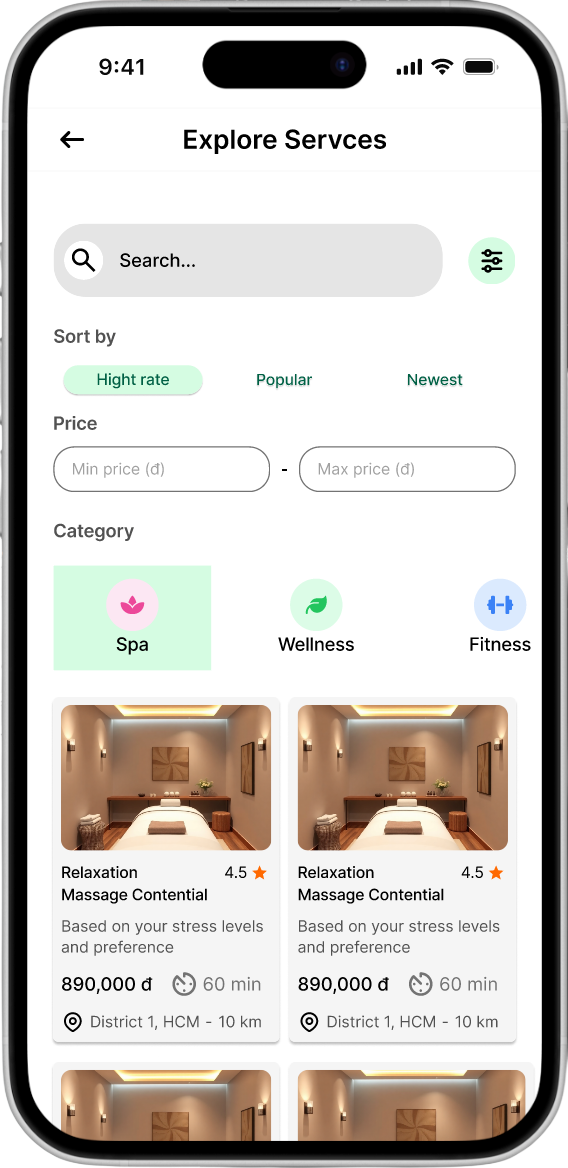
\includegraphics[width=\linewidth]{Images/uiux/navigation/explore_service.png}
        \caption{Explore Services}
    \end{subfigure}
    \hfill
    \begin{subfigure}[b]{0.24\textwidth}
        \centering
        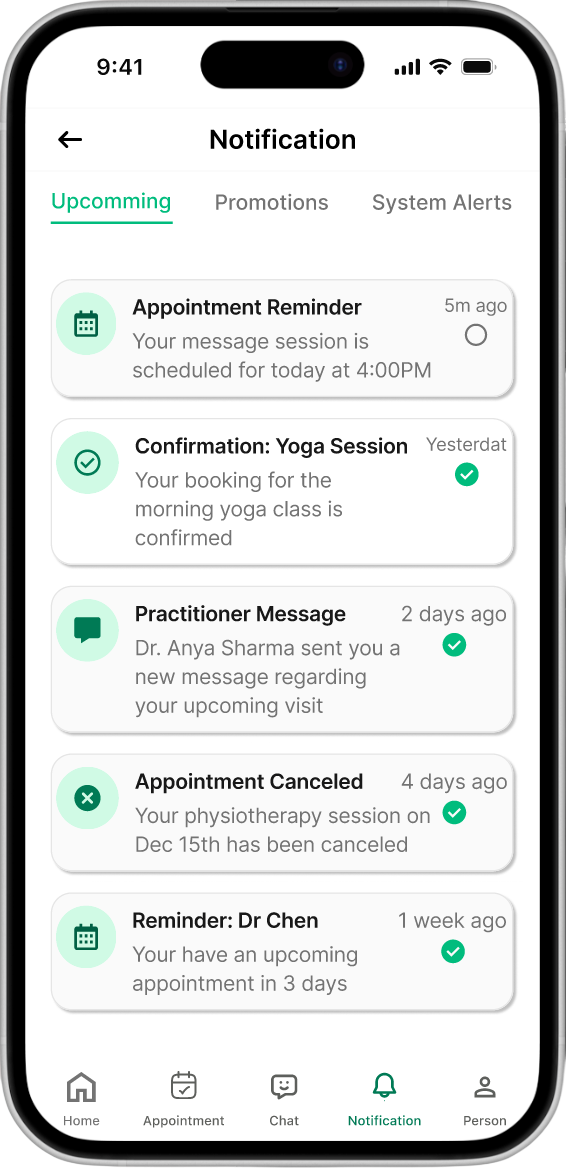
\includegraphics[width=\linewidth]{Images/uiux/navigation/notification.png}
        \caption{Notification}
    \end{subfigure}
    
    \vspace{1em}
    
    % --- Hàng 2 ---
    \begin{subfigure}[b]{0.24\textwidth}
        \centering
        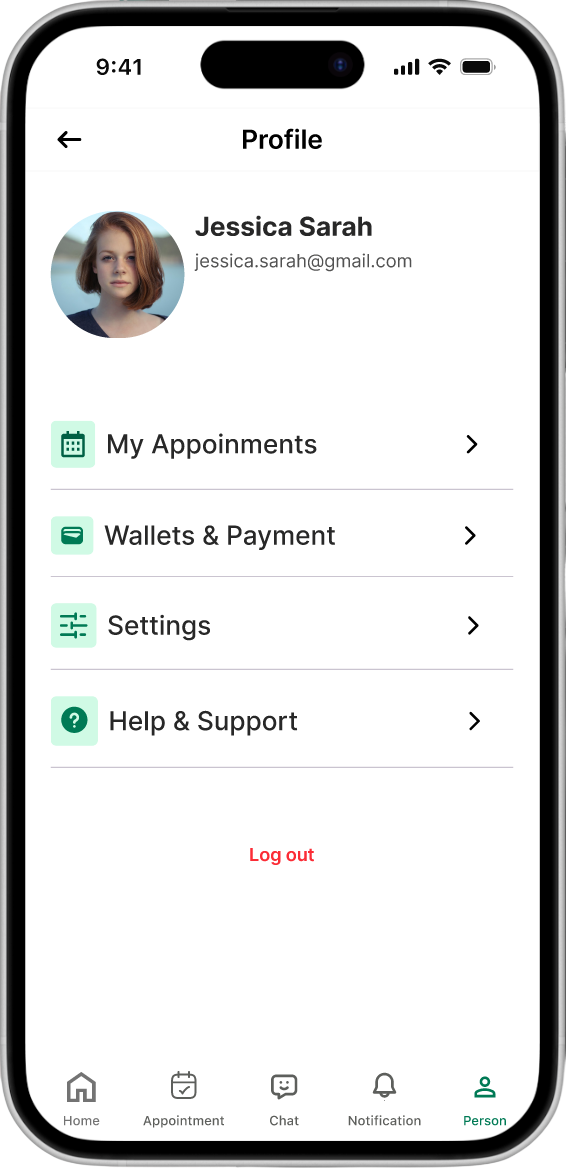
\includegraphics[width=\linewidth]{Images/uiux/navigation/personal.png}
        \caption{Personal Profile}
    \end{subfigure}
    \hfill
    \begin{subfigure}[b]{0.24\textwidth}
        \centering
        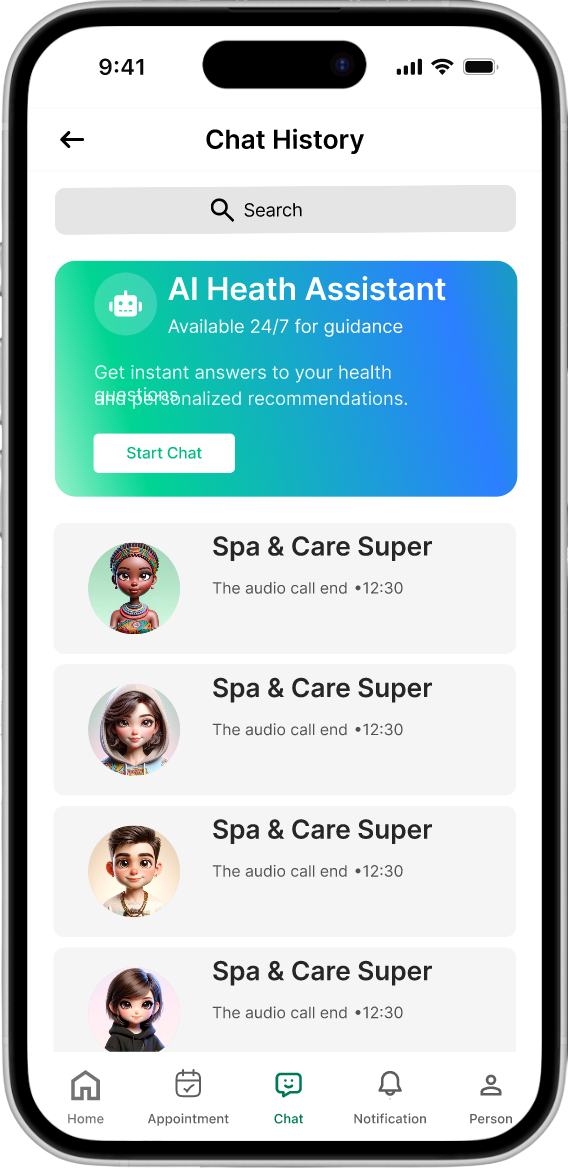
\includegraphics[width=\linewidth]{Images/uiux/navigation/chat_history.png}
        \caption{Chat History}
    \end{subfigure}
    \hfill
    \begin{subfigure}[b]{0.24\textwidth}
        \centering
        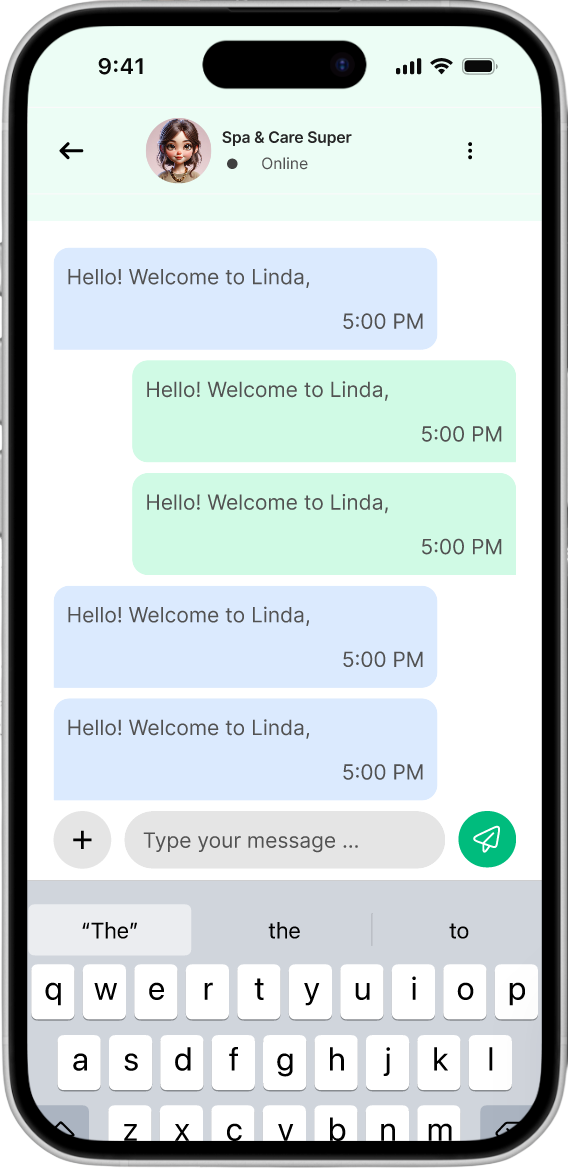
\includegraphics[width=\linewidth]{Images/uiux/navigation/chat_box.png}
        \caption{Chat Box}
    \end{subfigure}
    \hfill
    \begin{subfigure}[b]{0.24\textwidth}
    \end{subfigure}
    
    \vspace{1em}
    \caption{Giao diện Navigation}
\end{figure}

\subsection{Appointment - Đặt lịch hẹn}
\begin{figure}[H]
    \centering
    
    % --- Hàng 1 ---
    \begin{subfigure}[b]{0.24\textwidth}
        \centering
        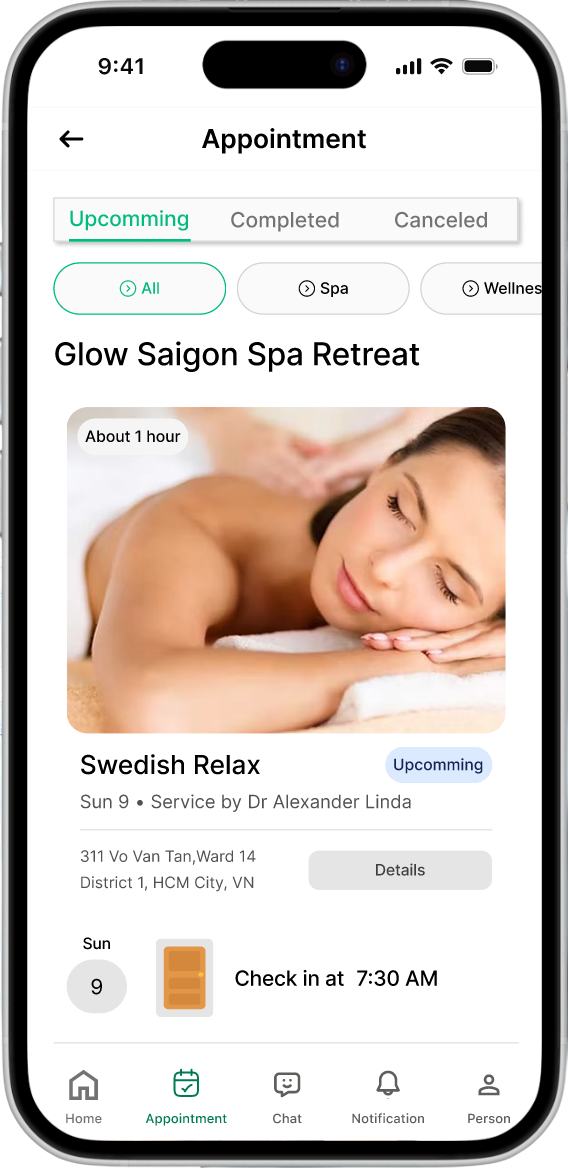
\includegraphics[width=\linewidth]{Images/uiux/appointment/appointment_1.png}
        \caption{Appointment Step 1}
    \end{subfigure}
    \hfill
    \begin{subfigure}[b]{0.24\textwidth}
        \centering
        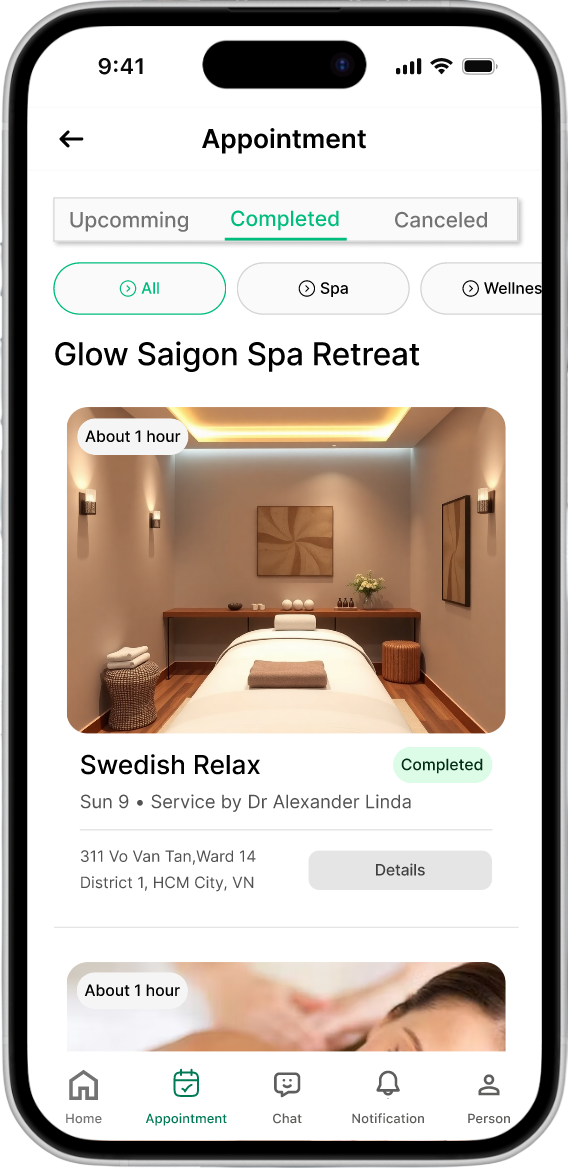
\includegraphics[width=\linewidth]{Images/uiux/appointment/appointment_2.png}
        \caption{Appointment Step 2}
    \end{subfigure}
    \hfill
    \begin{subfigure}[b]{0.24\textwidth}
        \centering
        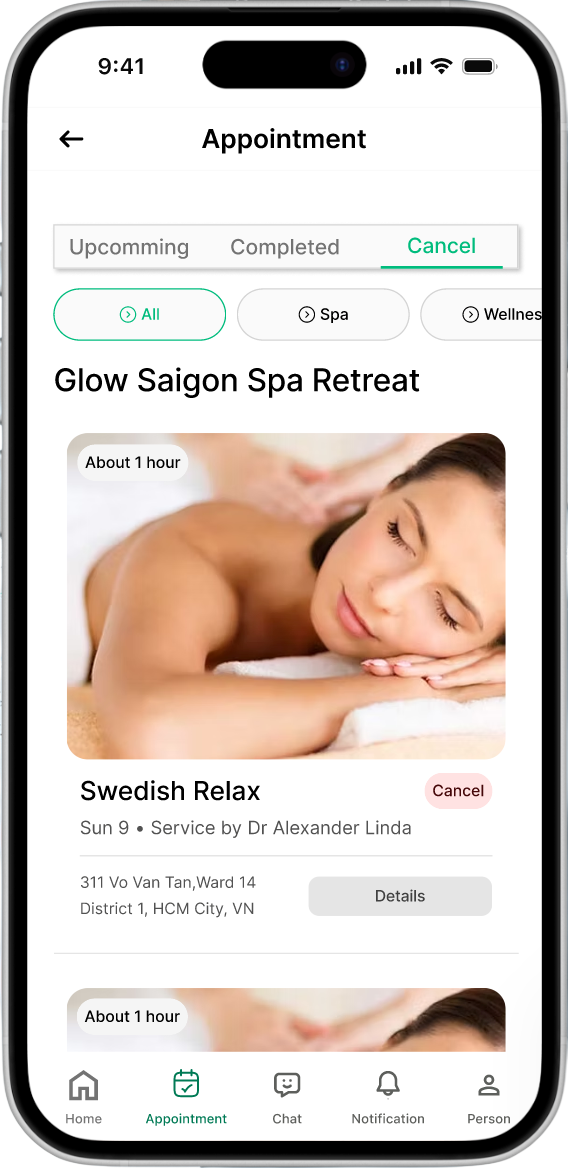
\includegraphics[width=\linewidth]{Images/uiux/appointment/appointment_3.png}
        \caption{Appointment Step 3}
    \end{subfigure}
    \hfill
    \begin{subfigure}[b]{0.24\textwidth}
        \centering
        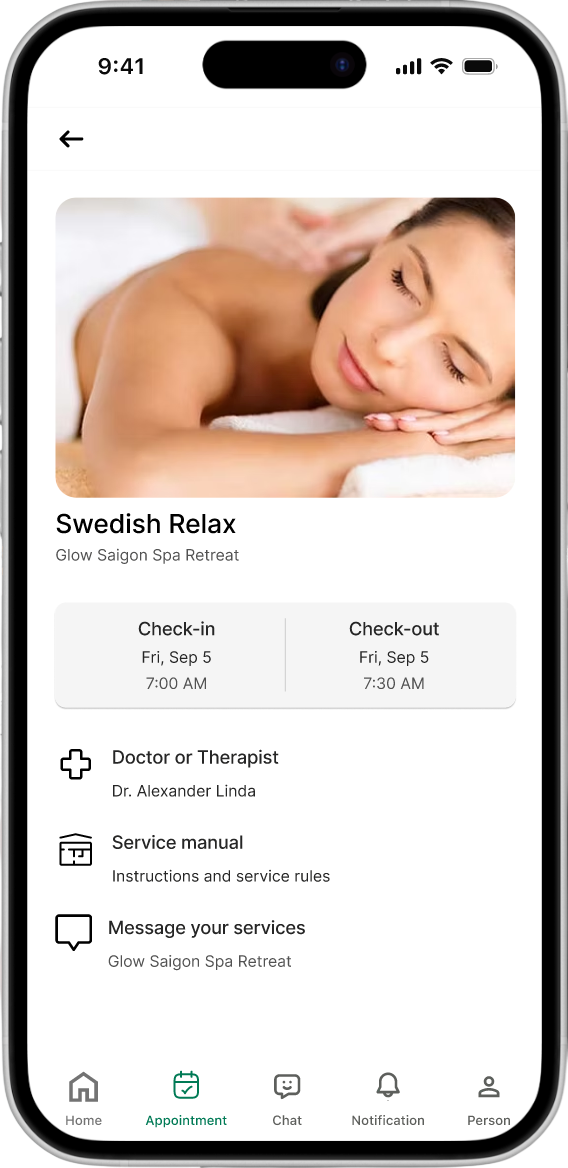
\includegraphics[width=\linewidth]{Images/uiux/appointment/appointment_details.png}
        \caption{Appointment Details}
    \end{subfigure}
    
    \vspace{1em}
    
    % --- Hàng 2 ---
    \begin{subfigure}[b]{0.24\textwidth}
        \centering
        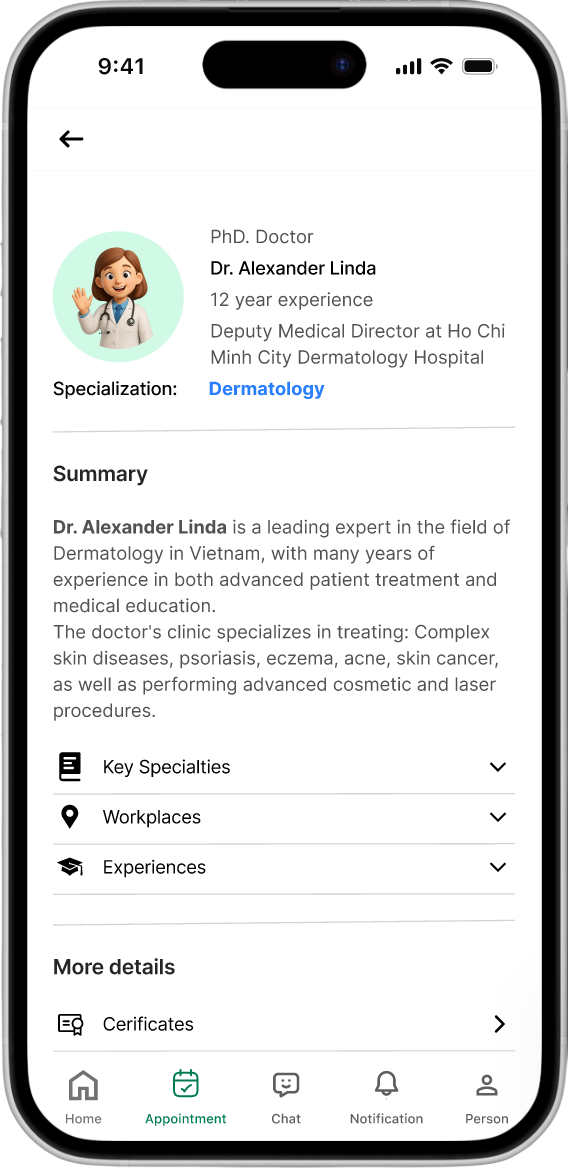
\includegraphics[width=\linewidth]{Images/uiux/appointment/doctor_detail.png}
        \caption{Doctor Detail}
    \end{subfigure}
    \hfill
    \begin{subfigure}[b]{0.24\textwidth}
        \centering
        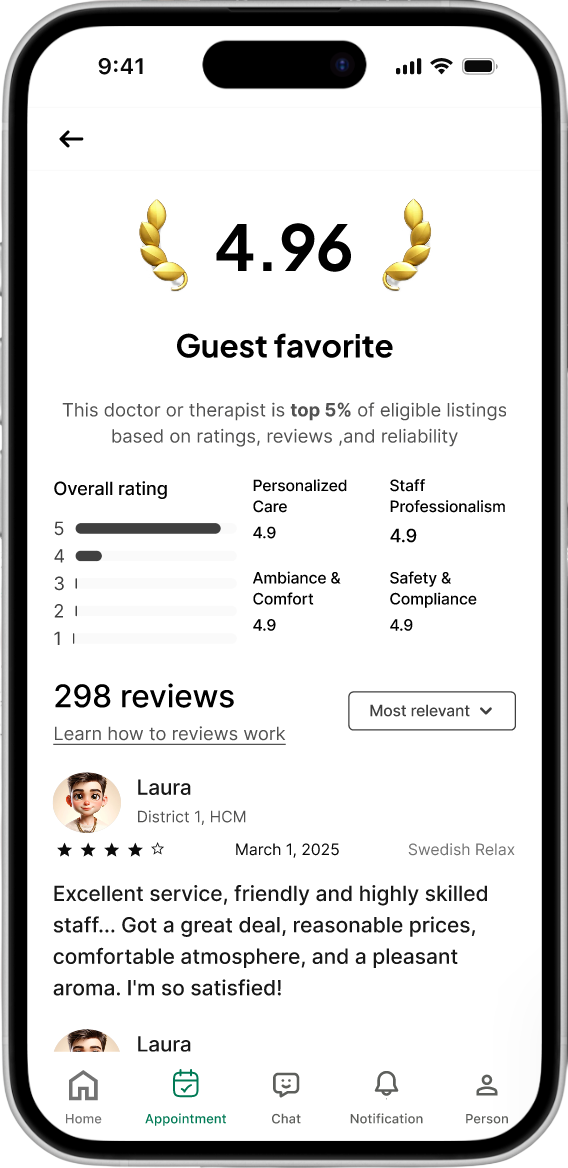
\includegraphics[width=\linewidth]{Images/uiux/appointment/review_detail.png}
        \caption{Review Detail}
    \end{subfigure}
    \hfill
    \begin{subfigure}[b]{0.24\textwidth}
    \end{subfigure}
    \hfill
    \begin{subfigure}[b]{0.24\textwidth}
    \end{subfigure}
    
    \vspace{1em}
    \caption{Giao diện Appointment}
\end{figure}

\subsection{AI Chat - Trợ lý AI}
\begin{figure}[H]
    \centering
    
    % --- Hàng 1 ---
    \begin{subfigure}[b]{0.24\textwidth}
        \centering
        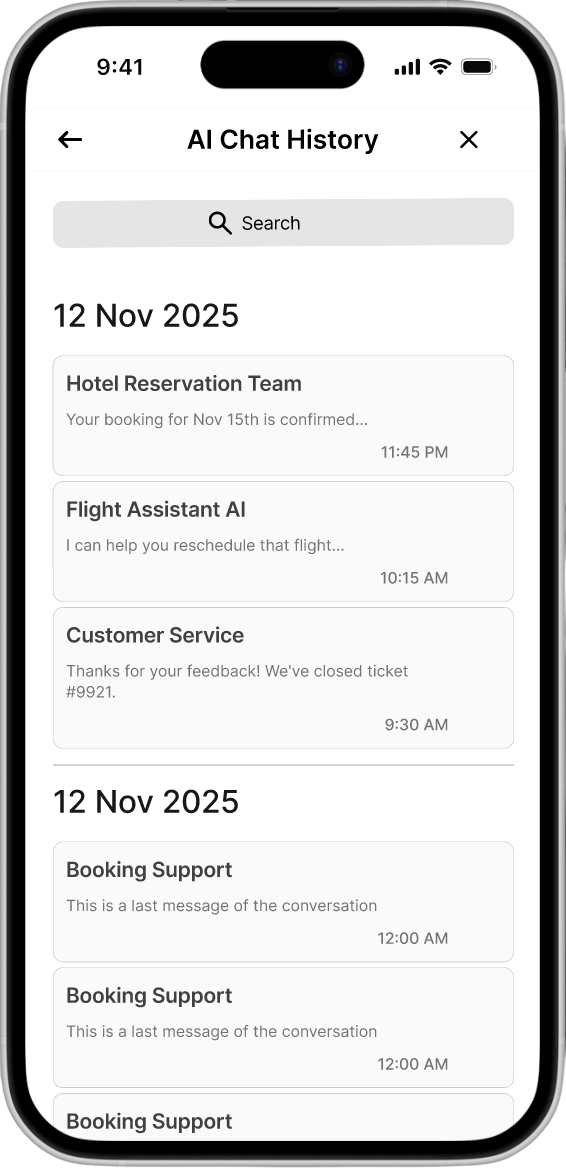
\includegraphics[width=\linewidth]{Images/uiux/ai_chat/aichat_session.png}
        \caption{AI Chat Session}
    \end{subfigure}
    \hfill
    \begin{subfigure}[b]{0.24\textwidth}
        \centering
        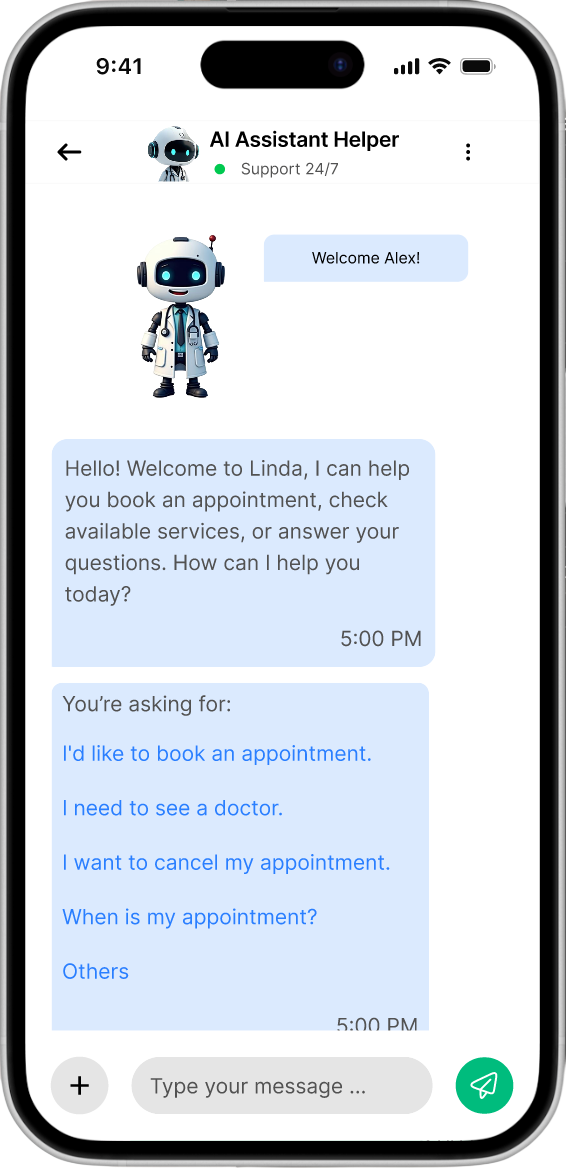
\includegraphics[width=\linewidth]{Images/uiux/ai_chat/aichat_box_1.png}
        \caption{AI Chat Box 1}
    \end{subfigure}
    \hfill
    \begin{subfigure}[b]{0.24\textwidth}
        \centering
        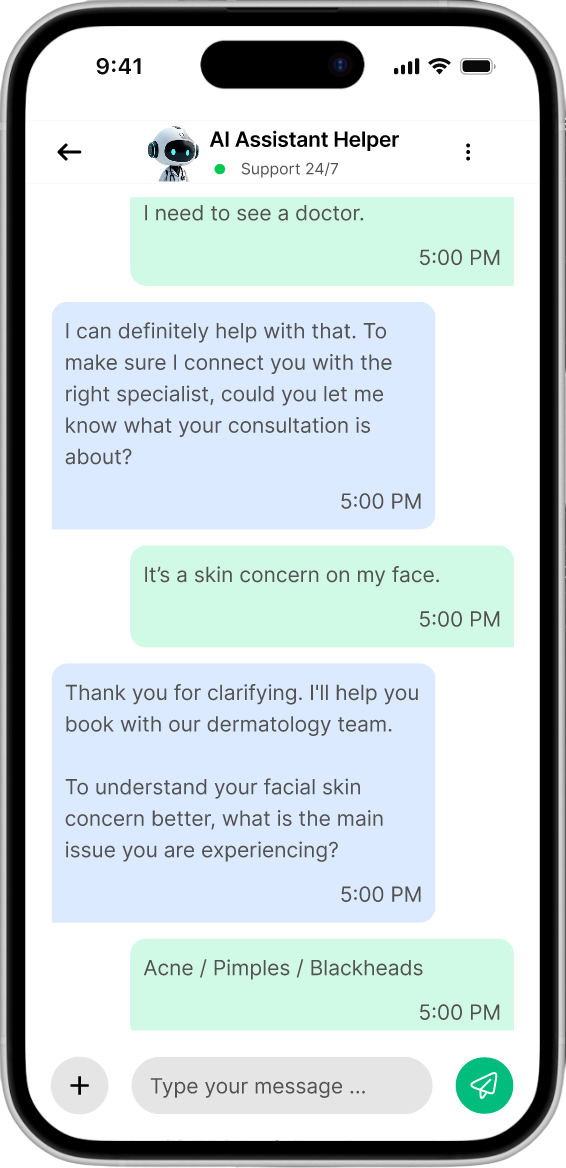
\includegraphics[width=\linewidth]{Images/uiux/ai_chat/aichat_box_2.png}
        \caption{AI Chat Box 2}
    \end{subfigure}
    \hfill
    \begin{subfigure}[b]{0.24\textwidth}
        \centering
        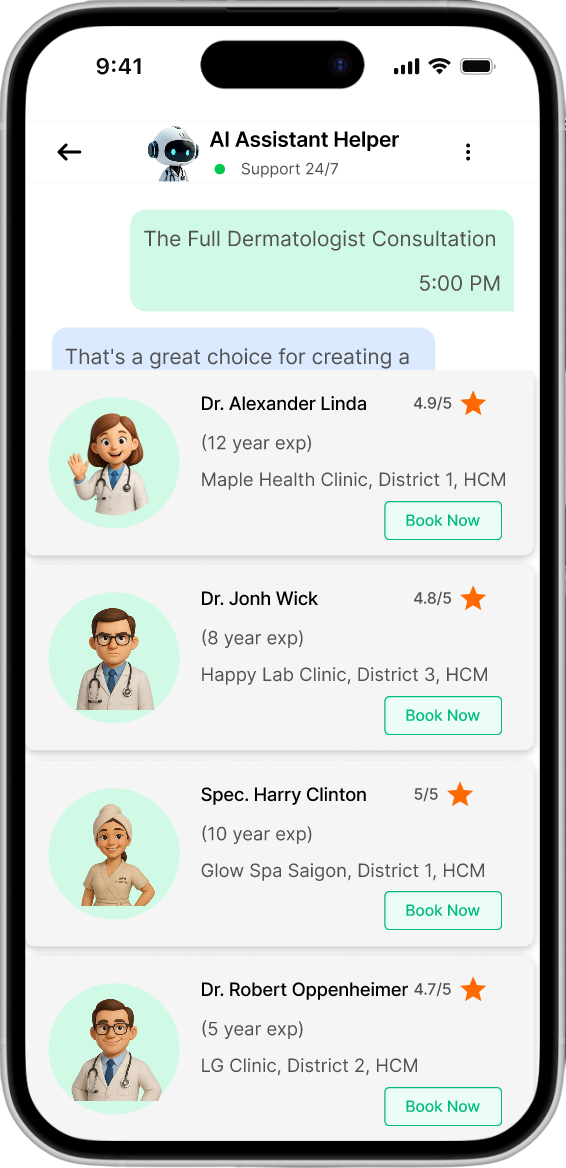
\includegraphics[width=\linewidth]{Images/uiux/ai_chat/aichat_box_3.png}
        \caption{AI Chat Box 3}
    \end{subfigure}
    
    \vspace{1em}
    
    % --- Hàng 2 ---
    \begin{subfigure}[b]{0.24\textwidth}
        \centering
        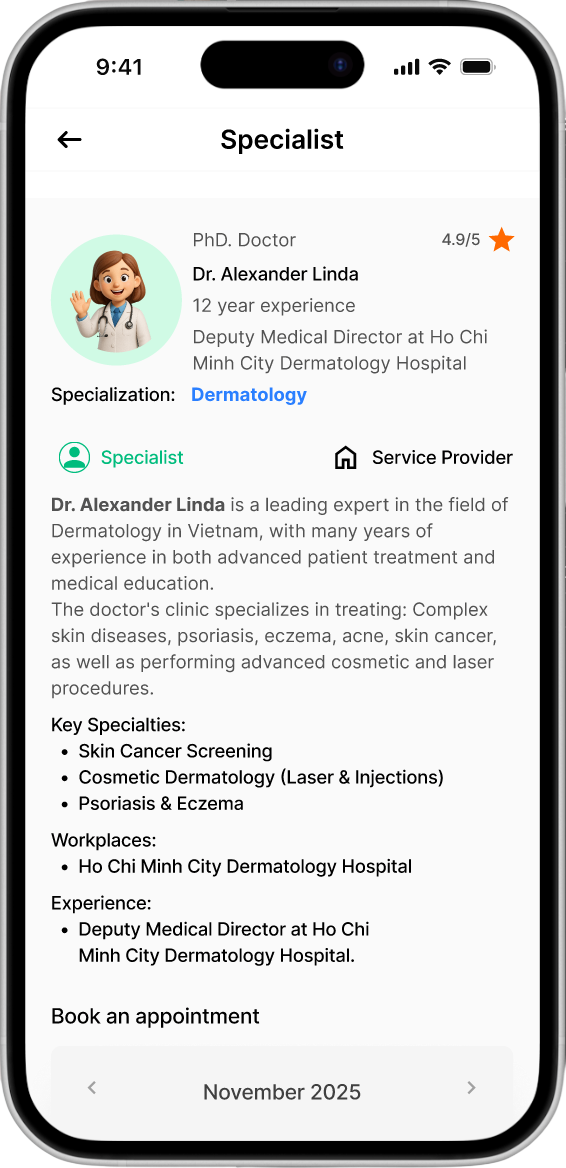
\includegraphics[width=\linewidth]{Images/uiux/ai_chat/aichat_box_4.png}
        \caption{AI Chat Box 4}
    \end{subfigure}
    \hfill
    \begin{subfigure}[b]{0.24\textwidth}
        \centering
        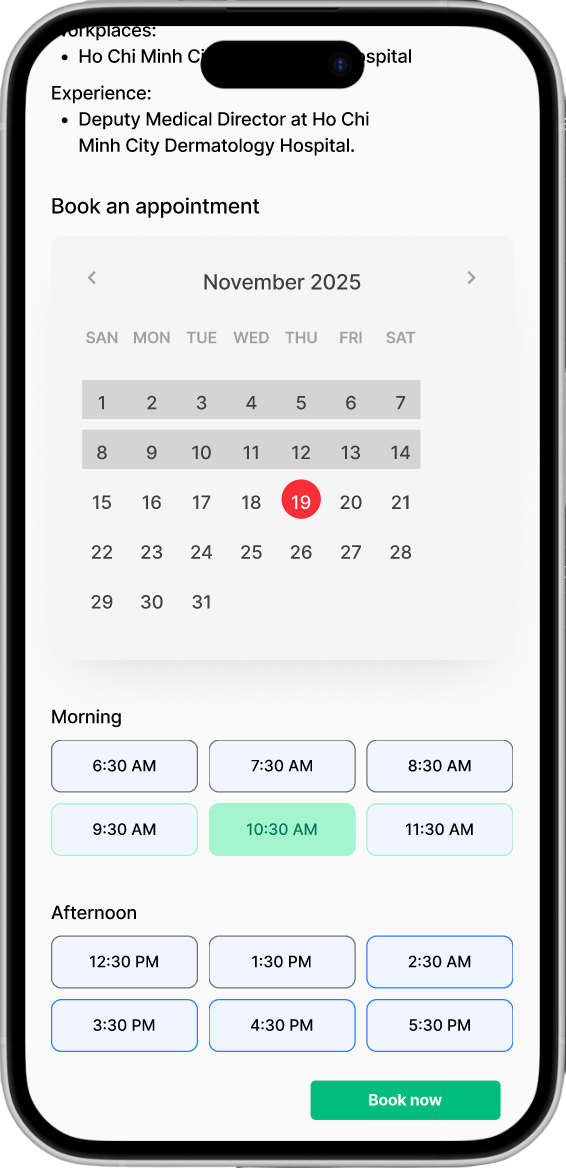
\includegraphics[width=\linewidth]{Images/uiux/ai_chat/aichat_box_5.png}
        \caption{AI Chat Box 5}
    \end{subfigure}
    \hfill
    \begin{subfigure}[b]{0.24\textwidth}
    \end{subfigure}
    \hfill
    \begin{subfigure}[b]{0.24\textwidth}
    \end{subfigure}
    
    \vspace{1em}
    \caption{Giao diện AI Chat}
\end{figure}

\section{Phần AI – Thiết kế}
\subsection{Thu thập và tiền xử lý dữ liệu}

Dữ liệu phục vụ các pipeline AI trong mã nguồn hiện tại được phân theo từng dịch vụ như sau.

\begin{itemize}
    \item \textbf{RAG Chatbot:} Kho tri thức gồm các tài liệu PDF; khi khởi động dịch vụ, toàn bộ PDF trong thư mục tri thức được đọc song song, loại bỏ ký tự ngoài ASCII (UTF-8), sau đó chia nhỏ bằng \textit{Recursive Character Text Splitter} với độ dài đoạn 300 ký tự và không chồng lấp giữa các đoạn.
    \item \textbf{Recommender (vector search):} Danh mục dịch vụ nguồn đọc từ tệp JSON; mỗi bản ghi được ghép thành một văn bản gồm tên và mô tả, gắn metadata \texttt{service\_id} và \texttt{category}, rồi được embedding và lưu vào Chroma persistent để truy vấn tương đồng.
    \item \textbf{Recommender Home (hồ sơ người dùng):} Dịch vụ gợi ý trang chủ đọc PostgreSQL: khảo sát người dùng lưu trong trường JSON trên bảng tài khoản (chuẩn hóa thành ba nhóm \textit{goals}, \textit{interests}, \textit{health\_conditions}), đồng thời có thể đọc hồ sơ cá nhân (tên, ngày sinh suy ra tuổi, v.v.). Danh sách mã dịch vụ đã dùng được dự kiến lấy từ lịch sử đơn hàng nhưng trong triển khai hiện tại luôn trả về rỗng cho đến khi tích hợp bảng đơn hàng.
    \item \textbf{NER / PreFilter:} Dịch vụ tải cache địa điểm và dữ liệu phục vụ lọc từ cơ sở dữ liệu quan hệ khi khởi động; hỗ trợ truy vấn không gian (PostGIS) khi có ngữ cảnh khoảng cách hợp lệ.
\end{itemize}

\subsection{Thiết kế hệ thống NER/PreFilter}

\subsubsection{Mục tiêu thiết kế và vai trò trong pipeline}

NER Service được thiết kế như một vi dịch vụ độc lập để tiếp nhận truy vấn ngôn ngữ tự nhiên, trích xuất thực thể và chuyển đổi thành điều kiện lọc cho tầng gợi ý. Trong pipeline hội thoại, dịch vụ này đóng vai trò \textit{pre-filtering gate}: giảm không gian tìm kiếm của recommender trước khi đưa vào bước xếp hạng ngữ nghĩa.

Các endpoint chính gồm:
\begin{itemize}
    \item \texttt{/ner/extract}: trả danh sách thực thể đã chuẩn hóa.
    \item \texttt{/prefilter/search}: chạy luồng extract $\rightarrow$ normalize $\rightarrow$ spatial filter và trả danh sách \texttt{service\_id} phù hợp.
\end{itemize}

\subsubsection{Kiến trúc Hybrid NER}

Hệ thống áp dụng kiến trúc lai (Hybrid NER), kết hợp nhiều kỹ thuật để cân bằng giữa độ chính xác và tính ổn định vận hành:
\begin{itemize}
    \item \textbf{LLM-based extraction (Gemini):} xử lý tốt các thực thể ngữ nghĩa như loại hình dịch vụ và cụm ý định phức tạp.
    \item \textbf{Rule-based extraction:} parser cục bộ cho dữ liệu định lượng giúp kiểm soát tốt operator và đơn vị đo.
    \item \textbf{NLP + Dictionary fallback:} underthesea, keyword scan và bộ dò địa danh (Aho-Corasick hoặc n-gram fallback) để duy trì khả năng hoạt động khi LLM lỗi hoặc timeout.
\end{itemize}

\subsubsection{Thiết kế luồng xử lý thực thể}

Một truy vấn đầu vào được xử lý theo chuỗi bước:
\begin{enumerate}
    \item \textbf{Gemini extraction}: lấy thực thể thô theo schema JSON.
    \item \textbf{Local enrichment}: chạy bổ sung underthesea, keyword scan và location fallback.
    \item \textbf{Numeric policy}:
    \begin{itemize}
        \item \texttt{PRICE}: \textbf{Gemini-first}, chỉ fallback regex local khi Gemini không trả PRICE.
        \item \texttt{DISTANCE}: \textbf{Gemini-first}, fallback local deterministic extractor khi Gemini không trả DISTANCE.
    \end{itemize}
    \item \textbf{Normalization}: ánh xạ về các trường chuẩn như \texttt{business\_type}, \texttt{location\_code}, \texttt{operator}, \texttt{amount}.
    \item \textbf{Query building}: tổng hợp tham số lọc cho truy vấn PostgreSQL/PostGIS.
\end{enumerate}

\subsubsection{Chiến lược tối ưu và độ bền hệ thống}

Để đáp ứng yêu cầu thời gian thực, thiết kế dịch vụ ưu tiên tính ổn định theo các cơ chế sau:
\begin{itemize}
    \item \textbf{LRU query cache}: lưu truy vấn gần nhất để giảm chi phí xử lý lặp.
    \item \textbf{Startup preload}: nạp cache vị trí từ database ngay khi khởi động.
    \item \textbf{Stale-while-revalidate}: khi refresh cache thất bại, vẫn dùng dữ liệu cũ để tránh gián đoạn.
    \item \textbf{Confidence gating}: lọc confidence thấp cho các thực thể ngữ nghĩa trọng yếu nhằm giảm false positive trước pha truy vấn.
\end{itemize}

\subsubsection{Thiết kế schema trao đổi dữ liệu}

Contract giữa Gateway và NER Service dùng mô hình dữ liệu có cấu trúc để đảm bảo tính xác định khi chuyển sang điều kiện truy vấn:
\begin{itemize}
    \item Trường lõi: \texttt{type}, \texttt{value}, \texttt{confidence}.
    \item Trường chuẩn hóa theo miền: \texttt{business\_type}, \texttt{location\_code}, \texttt{location\_level}.
    \item Trường định lượng: \texttt{operator}, \texttt{amount}, \texttt{amount\_max}, \texttt{radius\_meters}.
\end{itemize}

Thiết kế này giúp quá trình kiểm thử, phân tích lỗi và hiệu chỉnh pipeline diễn ra minh bạch hơn, đồng thời giảm sai khác giữa môi trường đánh giá và môi trường vận hành thực tế.
% ============================================================
% THIẾT KẾ HỆ THỐNG
% ============================================================

\subsection{Thiết kế hệ thống RAG Chatbot}

\subsubsection{Luồng tích hợp tổng thể}

Trong kiến trúc microservices của hệ thống, dịch vụ chatbot không hoạt động độc lập mà được điều phối thông qua một \textbf{Gateway Service} trung tâm. Mỗi khi người dùng gửi tin nhắn, Gateway chịu trách nhiệm lưu trữ hội thoại vào PostgreSQL, nạp lại lịch sử hội thoại, phân tích ý định của người dùng thông qua mô hình \textit{Intent Classification}, và quyết định có cần kích hoạt hệ thống gợi ý dịch vụ hay không. Sau khi thu thập đầy đủ ngữ cảnh, Gateway tổng hợp payload và chuyển tiếp đến dịch vụ RAG để sinh câu trả lời. Phản hồi được trả về dưới dạng luồng SSE liên tục, cho phép giao diện người dùng hiển thị từng đoạn văn bản ngay khi được sinh ra.

Thứ tự xử lý trong một phiên hội thoại diễn ra theo trình tự: phân loại ý định $\rightarrow$ (nếu cần) gọi dịch vụ NER để trích xuất địa điểm $\rightarrow$ gọi dịch vụ gợi ý $\rightarrow$ gọi dịch vụ RAG kèm ngữ cảnh đã làm giàu $\rightarrow$ phát các SSE event về client.

\subsubsection{Pipeline RAG trong dịch vụ chatbot}

Dịch vụ RAG nhận payload từ Gateway gồm ba thành phần: lịch sử hội thoại đã định dạng, mô tả các dịch vụ liên quan (có thể rỗng nếu ý định không yêu cầu gợi ý), và câu hỏi hiện tại của người dùng. Pipeline xử lý nội bộ bao gồm:

\begin{enumerate}
    \item \textbf{Truy xuất ngữ cảnh:} Câu hỏi hiện tại được embedding thông qua lớp \texttt{HuggingFaceEmbeddings} của LangChain, ưu tiên thiết bị CUDA khi có. Hệ thống tìm kiếm trong vector store \textbf{ChromaDB} theo chế độ \textit{similarity} với $k = 10$ đoạn tài liệu liên quan nhất, sau đó ghép nội dung các đoạn thành một khối ngữ cảnh thống nhất.

    \item \textbf{Xây dựng prompt:} Hệ thống sử dụng một mẫu prompt quy định rõ vai trò trợ lý sức khỏe, thứ tự ưu tiên nguồn thông tin (lịch sử hội thoại $\rightarrow$ knowledge base $\rightarrow$ dịch vụ gợi ý $\rightarrow$ kiến thức chung), và các ràng buộc an toàn y tế. Mô tả dịch vụ chỉ được đưa vào prompt khi danh sách gợi ý không rỗng.

    \item \textbf{Sinh câu trả lời:} Mô hình ngôn ngữ \textbf{Llama-3.1-8B-Instruct} được tải với lượng tử hoá 4-bit (NF4, double quantization, compute dtype float16).

    \item \textbf{Trả về luồng:} Sau khi có câu trả lời đầy đủ, dịch vụ chatbot chia nhỏ văn bản thành các cụm từ và trả về dưới dạng \texttt{StreamingResponse} (plain text). Gateway nhận từng chunk và bọc thành SSE event kiểu \texttt{TOKEN} trước khi đẩy về client.
\end{enumerate}

Kho tri thức được xây dựng từ các tài liệu PDF của Tổ chức Y tế Thế giới (WHO) bao gồm hướng dẫn về bệnh tim mạch, đái tháo đường, huyết áp, sức khoẻ tâm thần và hoạt động thể chất. Tài liệu được đọc song song bằng multiprocessing, làm sạch ký tự không thuộc ASCII, và chia đoạn bằng \textit{RecursiveCharacterTextSplitter} với độ dài 300 ký tự, không chồng lấp. Vector store được dựng lại mỗi khi dịch vụ khởi động.

\subsubsection{Thiết kế SSE và phân tách trách nhiệm}

Hệ thống áp dụng kiến trúc phân tách rõ ràng giữa các tầng xử lý SSE. Tầng dữ liệu (\texttt{SSEEvent}) là một đối tượng thuần tuý chứa tên event và payload, hoàn toàn không phụ thuộc vào FastAPI hay HTTP. Tầng định dạng (\texttt{SSEFormatter}) chịu trách nhiệm encode theo chuẩn \texttt{text/event-stream}. Tầng adapter (\texttt{sse\_stream}) là cầu nối giữa async generator của orchestrator và \texttt{StreamingResponse} của FastAPI. Kiến trúc này đảm bảo orchestrator chỉ cần \texttt{yield SSEEvent} mà không cần biết bất kỳ chi tiết HTTP nào.

Hệ thống định nghĩa bốn loại event trong một phiên hội thoại:

\begin{itemize}
    \item \textbf{TOKEN}: Mỗi cụm từ được sinh ra, kèm \texttt{conversation\_id} và timestamp.
    \item \textbf{RECOMMENDATION}: Danh sách chi tiết dịch vụ gợi ý, phát sau khi luồng LLM kết thúc.
    \item \textbf{DONE}: Tín hiệu kết thúc phiên, kèm trạng thái \texttt{completed} hoặc \texttt{failed}.
    \item \textbf{ERROR}: Thông báo lỗi có cấu trúc, được phát trước \texttt{DONE} khi xảy ra ngoại lệ.
\end{itemize}

% ============================================================

\subsection{Thiết kế hệ thống gợi ý dịch vụ cá nhân hóa}

\subsubsection{Kiến trúc tổng thể}

Hệ thống gợi ý được thiết kế theo phương pháp \textbf{tìm kiếm ngữ nghĩa} (\textit{semantic similarity search}) trên không gian vector, không sử dụng collaborative filtering hay rule-based ranking. Toàn bộ logic gợi ý dựa trên khoảng cách cosine giữa vector biểu diễn nhu cầu người dùng và vector biểu diễn từng dịch vụ trong cơ sở dữ liệu vector.

Hệ thống phục vụ hai luồng gợi ý độc lập:

\begin{itemize}
    \item \textbf{Home Recommender}: Gợi ý trên trang chủ, dựa trên hồ sơ sức khoẻ người dùng lấy từ cuộc khảo sát ban đầu khi đăng ký tài khoản.
    \item \textbf{Chatbot Recommender}: Gợi ý theo ngữ cảnh hội thoại, dựa trên câu hỏi tự nhiên của người dùng, có thể kết hợp với danh sách dịch vụ ứng viên do NER Service cung cấp.
\end{itemize}

\subsubsection{Biểu diễn dịch vụ và xây dựng chỉ mục}

Mỗi dịch vụ trong cơ sở dữ liệu được biểu diễn dưới dạng một chuỗi văn bản kết hợp tên và mô tả. Chuỗi này được embedding bằng mô hình \textbf{sentence-transformers/paraphrase-multilingual-mpnet-base-v2} tạo ra vector 768 chiều. Metadata đi kèm mỗi vector gồm \texttt{service\_id} và \texttt{category}, phục vụ cho các truy vấn có lọc điều kiện.

Vector store sử dụng \textbf{ChromaDB} ở chế độ persistent, lưu trữ cục bộ trên đĩa. Quá trình xây dựng chỉ mục được thực hiện offline theo hai phương thức: tải dữ liệu từ tệp JSON mẫu (môi trường phát triển) hoặc truy vấn trực tiếp bảng \texttt{products} trong PostgreSQL (môi trường production). Hệ thống hỗ trợ thao tác \textit{upsert} để cập nhật dịch vụ mà không cần rebuild toàn bộ chỉ mục.

\subsubsection{Đồng bộ hoá dữ liệu thời gian thực}

Để đảm bảo vector store luôn đồng bộ với cơ sở dữ liệu nghiệp vụ, hệ thống triển khai một cơ chế lắng nghe sự kiện qua \textbf{Redis Pub/Sub}. Khi backend tạo mới, cập nhật hoặc xoá một dịch vụ, một sự kiện tương ứng được publish lên Redis. Dịch vụ recommender lắng nghe các kênh này và phản ứng bằng cách upsert hoặc xoá bản ghi trong vector store, đảm bảo tính nhất quán giữa dữ liệu nghiệp vụ và chỉ mục vector mà không cần can thiệp thủ công.

\subsubsection{Xây dựng truy vấn}

\paragraph{Home Recommender}
Truy vấn được xây dựng bằng cách nối các danh sách từ hồ sơ người dùng: tình trạng sức khoẻ, sở thích, mục tiêu và văn bản mô tả của các dịch vụ người dùng đã sử dụng trước đây (lấy từ vector store theo ID). Chuỗi tổng hợp này sau đó được embedding để tìm kiếm các dịch vụ có ngữ nghĩa tương đồng nhất.

\paragraph{Chatbot Recommender}
Câu hỏi tự nhiên của người dùng được embedding trực tiếp mà không qua bước tiền xử lý phức tạp. Khi NER Service cung cấp danh sách \texttt{service\_id} ứng viên dựa trên địa điểm hoặc loại hình dịch vụ được trích xuất từ câu hỏi, hệ thống bổ sung điều kiện lọc metadata vào truy vấn ChromaDB, thu hẹp không gian tìm kiếm và tăng độ chính xác gợi ý.

\subsubsection{Làm giàu kết quả và tích hợp với Gateway Service}

Recommender Service trả về danh sách \texttt{service\_id} và điểm tương đồng. Gateway nhận kết quả này và thực hiện bước làm giàu thông tin: tra cứu chi tiết từng dịch vụ (tên, mô tả, giá, đánh giá, lịch trống, vị trí) để chuẩn bị cho hai mục đích song song — đưa mô tả dạng văn bản vào prompt LLM giúp chatbot phản hồi có ngữ cảnh, và đưa thông tin đầy đủ vào SSE event \texttt{RECOMMENDATION} để giao diện hiển thị thẻ dịch vụ.

% ============================================================

\subsection{Thiết kế hệ thống Intent Classification}

\subsubsection{Mục tiêu và vị trí trong pipeline}

Bài toán phân loại ý định được thiết kế là \textbf{phân loại nhị phân}: xác định liệu tin nhắn người dùng có yêu cầu gợi ý dịch vụ hay không. Kết quả phân loại quyết định luồng xử lý tiếp theo trong Gateway — nếu nhãn dương, Gateway tiến hành gọi NER Service và Recommender Service trước khi gọi RAG; nếu nhãn âm, Gateway bỏ qua các bước đó và gọi thẳng dịch vụ chatbot.

\subsubsection{Kiến trúc mô hình}

Mô hình sử dụng kiến trúc hai tầng:

\begin{enumerate}
    \item \textbf{Encoder:} SentenceTransformer mã hoá câu đầu vào thành vector biểu diễn ngữ nghĩa cố định chiều. Mô hình encoder được huấn luyện với \texttt{all-MiniLM-L6-v2} và lưu cục bộ cùng mã nguồn để đảm bảo hoạt động offline, chạy trên CPU khi suy luận.
    \item \textbf{Bộ phân lớp:} Hồi quy logistic (scikit-learn) nhận vector từ encoder và dự đoán nhãn nhị phân (0: không cần gợi ý, 1: cần gợi ý). Trọng số được lưu dưới dạng tệp pickle và nạp theo cơ chế singleton để tránh tải lại nhiều lần trong vòng đời ứng dụng.
\end{enumerate}

Mô hình được huấn luyện trên tập dữ liệu 1000 samples, với các mẫu dương tính là các câu hỏi yêu cầu tìm kiếm, gợi ý dịch vụ hoặc mô tả triệu chứng, và các mẫu âm tính là các câu chào hỏi, hỏi thông tin y tế chung, hoặc yêu cầu quản lý lịch hẹn.
